% Author of the LaTeX class is Lennart Franked.
% Main author of the original thesis-template contents is Stefan Forsstrom at Mid Sweden University.
% This repository keeps the MIUN LaTeX template as the output format and replaces
% the example body text with a report-writing skeleton for the narrowed new-yacoub thesis.

\documentclass[english]{miunthesis}
\usepackage{csquotes}
\usepackage{booktabs}
\usepackage{float}
\usepackage{newfloat}
\usepackage[]{appendix}
\usepackage{tabularx}
\usepackage{array}
\usepackage{ragged2e}
\usepackage{xurl}
\usepackage{seqsplit}

\newcommand{\codepath}[1]{\texttt{\seqsplit{#1}}}
\newcolumntype{Y}{>{\RaggedRight\arraybackslash}X}
\newcolumntype{L}[1]{>{\RaggedRight\arraybackslash}p{#1}}

\graphicspath{{Figures/}}
\addbibresource{literature.bib}

\title{[CHECK VALUE: final thesis title]}
\subtitle{PC-hosted n8n, Python middleware, shared contracts, and Tier 1.5 Raspberry Pi validation}
\author{[CHECK VALUE: author name]}

\projecttype{[CHECK VALUE: DT099G thesis project type]}

\fieldofstudy{Computer Engineering}
\coursecredits{15 hp}

\supervisor{[CHECK VALUE: supervisor name]}
\examiner{[CHECK VALUE: examiner name]}

\coursecode{DT099G}
\registrationnr{[CHECK VALUE: registration number]}

\studyprogramme{[CHECK VALUE: study programme or course]}

\begin{document}
  \maketitle
  \pagenumbering{roman}
  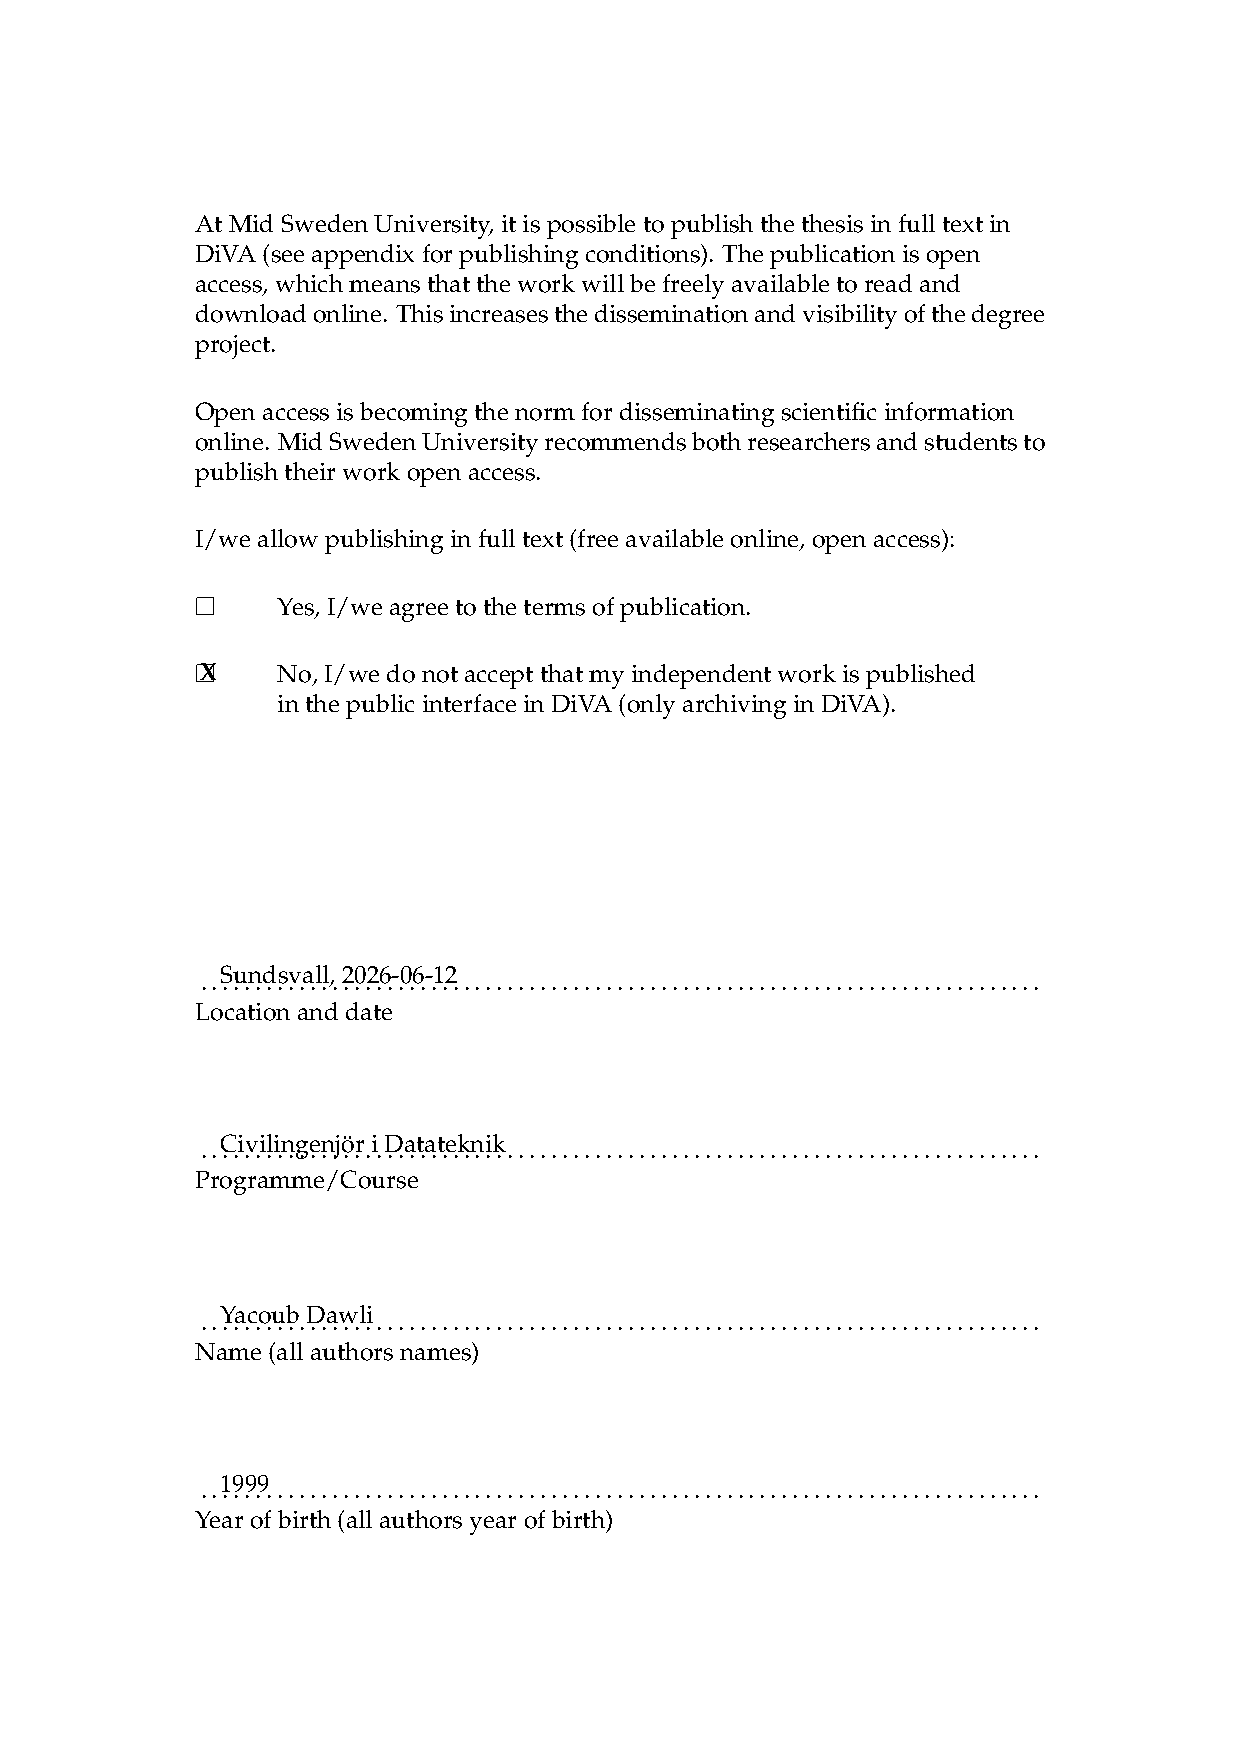
\includepdf[pages=1]{Diva_publish.pdf}
  \newpage
  \printabstract

  \section*{\translate{Acknowledgements}/\translate{Foreword}}\label{sec:acknowledgements}
\phantomsection
\addcontentsline{toc}{section}{\translate{Acknowledgements}}
% Optional MIUN front matter.
% What to write: brief thanks if the author wants to include them.
% Source files: none required.
% Missing checks: [CHECK VALUE: decide whether to keep or remove this optional section].

  \newpage

  \tableofcontents
  \newpage

  \phantomsection
  \listoffigures
  \addcontentsline{toc}{section}{\translate{List of Figures}}
  \newpage

  \phantomsection
  \listoftables
  \addcontentsline{toc}{section}{\translate{List of Tables}}
  \newpage

  \phantomsection
  \listofalgorithms
  \addcontentsline{toc}{section}{\translate{List of Algorithms}}
  \newpage

  \section*{\translate{Terminology}/\translate{Notation}}\label{sec:terminology}
\phantomsection
\addcontentsline{toc}{section}{Terminology / Notation}
% What to write: alphabetical definitions of terms that recur across the thesis.
% Main sources: README.md, docs/architecture/README.md, shared_interfaces/json-schema/*.json,
% docs/decisions.md, evaluation/metrics/metrics-schema.md.
% Missing checks: [CHECK VALUE: finalize terminology after Chapters 4-6 are drafted].

\begin{table}[ht!]
  \caption{Planned terminology entries to finalize during drafting.}
  \label{tab:terminology-planned}
  \begin{tabular}{@{}p{0.25\linewidth}p{0.65\linewidth}@{}}
    \toprule
    Term & Meaning to define in the final report \\
    \midrule
    API & [CHECK VALUE: define consistently with middleware implementation.] \\
    CSV & [CHECK VALUE: define as the evaluation result format.] \\
    GPIO & [CHECK VALUE: explain that real GPIO control was not implemented.] \\
    HITL & [CHECK VALUE: define human-in-the-loop approval as a minimum design element.] \\
    JSON contract & [CHECK VALUE: define using shared interface schemas.] \\
    LLM & [CHECK VALUE: define only as used by the minimal agent-enhanced workflow.] \\
    n8n & [CHECK VALUE: define as the self-hosted workflow automation engine.] \\
    Tier 1.5 validation & [CHECK VALUE: define as Raspberry Pi middleware/action validation while n8n remains on PC.] \\
    \bottomrule
  \end{tabular}
\end{table}

  \newpage
  \pagenumbering{arabic}
  \section{Introduction}\label{sec:intro}
% Chapter purpose: frame the thesis as a narrow, measurable proof-of-concept rather than a project diary.
% Course/template source: docs/course/DT099G information 2026-1 (1) (1).pdf and docs/templates/Miun ThesisTemplate 2026-01-21 (1).docx.
% Project source: docs/plans/implementation-plan.md, docs/ongoing/yacoub-scope.md, docs/decisions.md, README.md.
% Missing checks: [CHECK VALUE: final title, author metadata, supervisor name, examiner name].

\subsection{Background and Motivation}\label{subsec:background}
% Discuss: workflow automation, IoT-style event-action systems, and why a small controlled fan scenario is a useful proxy.
% Source files: README.md; docs/architecture/README.md; docs/report-notes/step-01-lock-scope.md.
% Figures/tables: no main figure required here; optionally refer forward to Figure~\ref{fig:final-architecture}.
% References needed: [REFERENCE NEEDED: IoT/edge computing source], [REFERENCE NEEDED: workflow automation/orchestration source], [REFERENCE NEEDED: n8n documentation].
% Missing checks: [CHECK VALUE: exact non-technical motivation and problem framing].

\subsection{Problem Statement}\label{subsec:problem-statement}
% Discuss: the investigated problem as a measurable integration/evaluation problem.
% Keep it narrow: PC-hosted Docker n8n, Python middleware, shared JSON contracts, simulated fan actions, CSV-based evaluation, and Tier 1.5 Raspberry Pi validation.
% Source files: docs/plans/implementation-plan.md; docs/decisions.md decisions D-001 through D-013; docs/report-notes/step-11-implementation-freeze.md.
% Figures/tables: no figure required.
% References needed: none beyond Chapter 2 theory references.
% Missing checks: [CHECK VALUE: final one-sentence problem statement].

\subsection{Aim}\label{subsec:aim}
% Discuss: aim of building and evaluating one complete vertical slice.
% Source files: docs/plans/implementation-plan.md; docs/ongoing/yacoub-scope.md; README.md.
% Figures/tables: no figure required.
% References needed: none.
% Missing checks: [CHECK VALUE: final aim statement aligned with RQ1-RQ3].

\subsection{Research Questions}\label{subsec:research-questions}
% Discuss: three measurable research questions only.
% Source files: user-approved updated research questions; docs/ongoing/research-questions.md may be historical and must be checked against this approved set.
% Figures/tables: no figure required.
% References needed: none.
% Missing checks: [CHECK VALUE: ensure the wording below remains the final supervisor-approved wording].

\begin{enumerate}
  \item \textbf{RQ1:} How accurately and consistently does the deterministic n8n workflow produce the expected fan action across the defined temperature test cases?
  \item \textbf{RQ2:} How accurately and consistently does the minimal agent-enhanced workflow produce contract-valid action output compared with the deterministic baseline?
  \item \textbf{RQ3:} What latency, resource, and deployment behavior is observed during local execution and Raspberry Pi Tier 1.5 middleware validation?
\end{enumerate}

\subsection{Scope and Limitations}\label{subsec:scope-limitations}
% Discuss: what is included and excluded at the start, before making claims.
% Must include: one scenario, simulated fan actions, PC-hosted n8n, middleware bridge, deterministic baseline, minimal agent-enhanced path, shared JSON contracts, minimum safety design, CSV evaluation, Tier 1.5 Pi validation.
% Must exclude: full n8n-on-Pi deployment, real GPIO hardware, production-grade safety enforcement, multi-agent architecture, large benchmarking, multiple devices/models, heavy observability stacks.
% Source files: docs/ongoing/yacoub-scope.md; docs/decisions.md; docs/report-notes/final-evidence-inventory.md.
% Figures/tables: optional scope table if the chapter needs clarity.
% References needed: none.
% Missing checks: [CHECK VALUE: confirm no later chapter overclaims beyond the frozen implementation].

\subsection{Contributions}\label{subsec:contributions}
% Discuss: concise technical contribution and author/supervisor roles.
% Use a CRediT-style list later:
% Conceptualization: author, with supervisor feedback.
% Methodology: author, with supervisor feedback.
% Software: author.
% Validation: author.
% Investigation: author.
% Data curation: author.
% Writing - original draft: author.
% Writing - review and editing: author, with supervisor feedback.
% Supervision: supervisor.
% Source files: docs/report-notes/step-11-implementation-freeze.md; docs/report-notes/final-evidence-inventory.md.
% Figures/tables: no figure required.
% References needed: none.
% Missing checks: [CHECK VALUE: supervisor name and final contribution wording].

\subsection{Usage of AI Tools in This Thesis}\label{subsec:ai-tools}
% Discuss: how AI tools supported planning, review, repair, report scaffolding, or text drafting, if applicable.
% Course/template source: docs/templates/Miun ThesisTemplate 2026-01-21 (1).docx requires this section in Chapter 1.
% Source files: AGENTS.md; .agents/ if relevant; this LaTeX skeleton creation; final author workflow notes.
% Figures/tables: no figure required.
% References needed: [REFERENCE NEEDED: course or university AI-use policy if required].
% Missing checks: [CHECK VALUE: exact AI tools used and final author responsibility statement].

\subsection{Division of Work / Author Contribution}\label{subsec:division-work}
% Discuss: which parts were performed by the author and what came from supervisor feedback.
% Source files: docs/report-notes/*.md; final evidence inventory; supervisor feedback in thesis-writing task.
% Figures/tables: no figure required.
% References needed: none.
% Missing checks: [CHECK VALUE: confirm whether this is a single-author thesis and whether external help must be named].

\subsection{Report Outline}\label{subsec:outline}
% Discuss: short chapter-by-chapter outline beginning with Chapter 2, per the MIUN template.
% Source files: this LaTeX skeleton and thesis/report-writing-map.md.
% Figures/tables: no figure required.
% References needed: none.
% Missing checks: [CHECK VALUE: update after final chapter titles are locked].

  \section{Theory and Related Work}\label{sec:theory}

This chapter presents the theoretical background needed to understand the proof-of-concept developed in this thesis. The focus is on workflow automation, IoT-style event-action systems, middleware boundaries, structured contracts, deterministic and agent-enhanced workflows, validation, and limited edge-hardware validation. The chapter does not attempt to survey all IoT platforms, all workflow engines, or all agent architectures. Instead, it introduces the concepts that are needed to justify and interpret the implemented system.

\subsection{Workflow Automation and Orchestration}\label{subsec:workflow-automation}

Workflow automation concerns the coordination of tasks, decisions, and integrations through an explicit process structure. A workflow can start from an event, apply decision logic, transform data, and call external systems. This makes workflow automation useful in event-action systems where the purpose is not only to compute a value, but to connect an incoming event to a controlled response. Workflow patterns are a well-established way of describing recurring control-flow structures such as branching, routing, and synchronization \cite{workflowPatternsAalst}.

In this thesis, workflow automation is used as an orchestration layer. The workflow engine receives a temperature event, evaluates the event, and calls middleware endpoints. n8n is the workflow platform used for this purpose. It provides a self-hostable workflow environment with nodes for triggers, data handling, and HTTP calls \cite{n8nDocs}. The choice of n8n is not treated as a comparison against other workflow tools; it is the concrete orchestration platform used to implement and evaluate the thesis architecture.

\subsection{IoT Event-Action Systems and Edge Computing}\label{subsec:iot-edge}

IoT systems commonly involve devices, sensors, network communication, data processing, and actions in the physical or operational environment. A sensor event may represent a temperature reading, a state change, or another observation that requires a response. The response may be an alert, a control action, or a decision to do nothing. This event-action pattern is central to the thesis scenario, where a temperature event is used to select a simulated fan action. Broader IoT research identifies this kind of connection between sensing, computation, and action as a core part of Internet of Things systems \cite{iotSurveyAtzori}.

Edge computing is relevant when some processing or action endpoint is moved closer to the device or environment rather than keeping all functionality in a central server or cloud system. Edge computing can reduce reliance on distant infrastructure and can support latency-sensitive or context-specific behavior \cite{edgeComputingSatyanarayanan}. In this thesis, Raspberry Pi is used only as limited edge-style hardware for middleware/action endpoint validation. Raspberry Pi is a small computing platform that can run software services and connect to hardware interfaces \cite{raspberryPiDocs}. The thesis does not evaluate a complete edge deployment; it uses Raspberry Pi to validate the middleware/action side of the architecture.

\subsection{Middleware and API Boundaries}\label{subsec:middleware-theory}

Middleware is useful when a system needs to separate decision logic from action execution. In an event-action architecture, the workflow should not necessarily be the component that directly controls hardware-facing behavior. A middleware/API layer can receive a structured action request, expose a small set of endpoints, and isolate workflow logic from the internal details of the action implementation. This separation makes the system easier to reason about because the workflow, contract, validation design, and action endpoint can be discussed as separate parts of the architecture \cite{fieldingRest2000,httpSemanticsRfc9110}.

In this thesis, the middleware/API boundary is especially important because both deterministic workflow output and agent-enhanced workflow output may lead to fan actions. Routing those actions through middleware prevents the workflow or agent step from being treated as direct hardware control. It also creates a location where simulated endpoints can later be replaced by physical device control, provided that additional validation and safety work is added.

\subsection{Structured Data, JSON Contracts, and Validation}\label{subsec:json-contracts}

Structured data formats reduce ambiguity between connected components. If a workflow emits only free text, the receiving system must infer the intended action. If the workflow emits a structured object, the receiving system can inspect fields, allowed values, and missing data more consistently. This is why the thesis uses JSON-style sensor and action contracts rather than relying on informal text output.

JSON Schema provides a vocabulary for describing and validating the structure of JSON data \cite{jsonSchemaDocs}. At a theory level, a schema can define required fields, allowed values, and whether unexpected fields are permitted. In an event-action system, this makes it possible to describe what a valid sensor event or action request should look like. In this thesis, structured contracts support predictable routing and provide a basis for discussing validation. They do not by themselves guarantee production safety, but they make the intended boundary explicit.

\subsection{Deterministic Workflows}\label{subsec:deterministic-workflows}

A deterministic workflow uses fixed logic to map inputs to outputs. Given the same input and the same workflow configuration, the expected decision path is the same. In the thesis scenario, the deterministic baseline uses a temperature threshold: a value at or above the threshold leads to \texttt{fan\_on}, while a lower value leads to \texttt{fan\_off}.

Deterministic workflows are useful as baselines because their behavior is transparent and inspectable. The rule can be stated directly, the expected output can be defined before execution, and deviations can be identified clearly. This makes the deterministic baseline important for evaluating the rest of the proof-of-concept. It shows whether the basic workflow, middleware, action endpoints, and evaluation harness work for the defined temperature cases before the agent-enhanced path is considered.

\subsection{Minimal Agent-Enhanced Workflows}\label{subsec:agent-enhanced-workflows}

An agent-enhanced workflow includes a decision step where a language model contributes to selecting or producing an action. In broader research, language-model agents may combine reasoning and acting by producing intermediate reasoning steps, using tools, and interacting with external environments \cite{reactYao2023}. This thesis uses a much smaller version of that idea. The agent-enhanced path contains a single LLM-based decision step that is expected to produce structured action output for the same temperature-to-fan scenario as the deterministic baseline.

The important theoretical point is not broad autonomy. The important point is that an LLM decision step can be placed inside a workflow, constrained by a prompt, and connected to a structured output pipeline. For this thesis, the output is expected to fit the action contract and route to the same middleware endpoints as the deterministic baseline. This allows the agent-enhanced workflow to be compared with the deterministic workflow without changing the action execution layer.

\subsection{Safety, Validation, and Human-in-the-Loop Concepts}\label{subsec:safety-hitl-theory}

When workflow or agent output can trigger actions, validation becomes important. A system should be able to distinguish between an allowed action, a malformed action, and a risky or unsupported action. In the thesis scenario, allowed actions are limited to the simulated fan actions, while malformed or unknown actions should not be treated as valid action requests.

Human-in-the-loop concepts are relevant when automation may require review before execution. Human involvement can help with cases where automated output is uncertain, risky, or outside the expected action set. Research on interactive machine learning emphasizes the role of humans in guiding and controlling machine-assisted systems \cite{humanInTheLoopAmershi2014}. In this thesis, the safety material remains a documented validation and approval design. It supports reasoning about allowed, blocked, and risky cases, but it is not evidence of production-grade runtime enforcement.

\subsection{Summary of Theory}\label{subsec:theory-summary}

The theory in this chapter supports the thesis architecture as a combination of workflow automation, IoT-style event-action logic, middleware separation, structured JSON contracts, deterministic baseline behavior, a constrained agent-enhanced decision step, validation concepts, and limited Raspberry Pi middleware validation. Together, these concepts explain why the implemented system is structured as a controlled workflow-to-action proof-of-concept rather than as a broad IoT platform or general multi-agent system.

  \section{Methodology}\label{sec:methodology}

This chapter describes how the thesis work was carried out and how the proof-of-concept system was evaluated. The method was chosen to match the defined proof-of-concept scope: one controlled temperature-to-fan scenario, two workflow decision modes, lightweight measurement, and Raspberry Pi middleware/action-endpoint validation.

\subsection{Research Approach}\label{subsec:research-approach}

The thesis uses a design-and-evaluate proof-of-concept approach. The work first defines a limited technical problem, then builds an artifact that addresses that problem, evaluates the artifact with defined test cases, and finally discusses the limitations of the evidence. The approach fits the thesis because the research questions are not answered only by theoretical comparison; they require an implemented system that can produce observable workflow behavior, action outputs, latency values, resource observations, and deployment evidence \cite{designScienceHevner,designSciencePeffers}.

The evaluated artifact is a focused workflow-to-action system with PC-hosted n8n, middleware-based action execution, structured contracts, and file-based evaluation evidence. The evaluation is therefore artifact-centered and scenario-based rather than a benchmark of many platforms, devices, or language models.

\subsection{Development Method}\label{subsec:development-method}

The implementation was developed through controlled stages. This staged method was used to reduce scope risk and keep each part of the system testable before adding the next one. The work first defined the evaluation scope, then implemented the runtime setup, middleware boundary, shared contracts, workflow modes, validation design, evaluation harness, and Raspberry Pi middleware validation.

Each stage introduced one necessary layer and produced evidence before the next layer was added. The runtime setup established the workflow execution environment. The middleware provided the action boundary. The shared contracts made the event and action payloads explicit. The workflow modes provided the deterministic and agent-enhanced comparison. The evaluation harness made the system measurable through CSV files, and the Raspberry Pi validation tested the middleware/action endpoint on separate hardware.


Once the evaluated system had produced enough evidence for the research questions, the implementation was kept stable during result reporting. Larger extensions, such as deeper Raspberry Pi deployment, physical hardware control, broader agent behavior, and larger-scale evaluation, were kept outside the evaluated implementation and are treated as future work.



\subsection{Evaluation Design}\label{subsec:evaluation-design}

The evaluation was designed around one temperature-to-fan scenario. The same input cases were used for the deterministic baseline workflow and the minimal agent-enhanced workflow so that the two modes could be compared on the same task. The evaluation also included documented safety and validation cases and a separate Raspberry Pi validation setup.

The deterministic baseline was evaluated by checking whether the fixed n8n threshold rule produced the expected fan action for the defined high- and low-temperature cases. The minimal agent-enhanced workflow was evaluated by checking whether the agent path produced the expected fan action and whether the observed output was contract-shaped, meaning that it contained the expected action fields and supported fan-action values for the defined cases. This check is distinguished from full runtime JSON Schema validation. The evaluation did not include a measured runtime schema-validation gate or logged pass/fail validation results for every action output. The safety and validation cases were evaluated as documented design cases: one allowed action, one malformed blocked action, and one risky or unsupported action that should not be executed directly. The Raspberry Pi validation evaluated whether PC-hosted n8n could call a Raspberry Pi-hosted middleware/action endpoint for the same temperature-to-fan scenario.

The defined high- and low-temperature workflow cases used in the evaluation are listed in Table~\ref{tab:method-test-cases}. Full repository paths for the dataset, scripts, and result files are listed in Appendix~\ref{sec:appendix-source-code}.

\begin{table}[H]
  \centering
  \caption{Defined workflow test cases.}
  \label{tab:method-test-cases}
  \begin{tabular}{@{}p{0.32\linewidth}p{0.22\linewidth}p{0.20\linewidth}p{0.16\linewidth}@{}}
    \toprule
    Test case type & Input temperature & Expected action & Mode \\
    \midrule
    High-temperature workflow case & 31.4 C & \texttt{fan\_on} & Deterministic and agent \\
    Low-temperature workflow case & 24.5 C & \texttt{fan\_off} & Deterministic and agent \\
    \bottomrule
  \end{tabular}
\end{table}

The safety cases in the dataset use action objects rather than temperature events. The allowed case contains a complete \texttt{fan\_on} action for \texttt{fan\_1}. The blocked case omits required fields. The risky case uses an unsupported \texttt{open\_window} action and an unknown target. These safety cases provide design evidence for the documented validation boundary rather than proof of production runtime enforcement.

\subsection{Metrics and Data Collection}\label{subsec:metrics-data-collection}

The evaluation records both behavioral and measurement-oriented fields. The behavioral fields include the expected action, observed action, success or failure, expected safety result, and observed safety result where applicable. The measurement fields include latency, CPU values where available, RAM values where available, and thermal observations where available. Contract-shaped output is considered where workflow or agent output is expected to follow the shared action object structure. This means that the observed output is checked against the expected fields and supported values at the report-evidence level, not that a full runtime JSON Schema validator was implemented and measured.

Data collection is CSV-based. Raw result rows and processed summaries are written to the evaluation result folders listed in Appendix~\ref{sec:appendix-source-code}. The collection script posts test payloads to the configured workflow webhook and records the raw result fields. For workflow modes, success is recorded when the HTTP request succeeds and the observed action matches the expected action. The script measures latency using Python timing around the webhook HTTP request. It also attempts best-effort CPU and RAM collection through Docker statistics when available \cite{dockerStatsDocs}. Thermal values are not fabricated; when no supported thermal source is available, the field is recorded as \texttt{not\_available}.

The aggregation script aggregates raw CSV files into processed latency, resource, safety-outcome, and baseline-versus-agent summaries. CSV is used as a simple tabular exchange format, with Python's standard \texttt{csv} module used by the scripts \cite{csvRfc4180,pythonCsvDocs}. These files support the Results chapter by separating raw observations from summarized comparison tables. The evaluation protocol also notes that safety-mode rows can document expected safety behavior without proving runtime enforcement unless enforcement logic is implemented and logged.

\subsection{Raspberry Pi Validation Method}\label{subsec:pi-validation-method}



Raspberry Pi validation was used to test the middleware/action endpoint on separate hardware, while n8n remained running on the PC. The PC-hosted n8n workflow called the Raspberry Pi middleware over HTTP.

The Raspberry Pi validation checks whether the middleware/action endpoint can run on the Raspberry Pi and be called over the network while the n8n workflow remains PC-hosted. In this setup, the Raspberry Pi represents the action-endpoint side of the architecture rather than the full workflow runtime. The fan action is simulated, so the validation focuses on networked middleware behavior and deployment observations rather than physical GPIO-based fan control.


The Raspberry Pi evidence was stored with the evaluation artifacts listed in Appendix~\ref{sec:appendix-source-code}. The method included the same high- and low-temperature fan cases, full workflow latency collection for the PC-to-Pi workflow path, supporting direct endpoint latency observations, CPU/RAM observations for the middleware process, and thermal observation from the Raspberry Pi evidence.

\subsection{Validity and Limitations of the Method}\label{subsec:method-validity-limitations}


The evaluation method is designed for a controlled proof-of-concept rather than broad benchmarking. The number of test cases is small because the thesis focuses on one temperature-to-fan scenario and compares the defined deterministic and agent-enhanced workflow paths under the same inputs. The results are evidence for the implemented workflow-to-action pipeline, not general performance claims for all n8n, IoT, or agentic AI systems.



The Raspberry Pi validation focuses on the middleware/action-endpoint side of the architecture while the n8n workflow remains PC-hosted. The fan action is simulated, so the method evaluates workflow behavior, contract-shaped action output, middleware routing, latency observations, and deployment evidence rather than physical GPIO-based fan control or production runtime safety. Full runtime schema validation and safety enforcement are outside the measured implementation.


	\subsection{Summary of Method}\label{subsec:method-summary}

The method supports the research questions by combining a controlled implementation artifact with repeatable, file-based evaluation evidence. It compares the two workflow decision modes under the same temperature cases, records action outcomes and measurements where available, and uses Raspberry Pi middleware validation as separate-hardware deployment evidence.

  \section{Choice of Approach / System Design}\label{sec:system-design}

This chapter explains the design choices that shaped the final proof-of-concept before the implementation details are presented. The purpose is to justify why the system was designed as a bounded workflow-to-action pipeline rather than as a broader automation platform, hardware project, or multi-agent system.

\subsection{Design Requirements and Constraints}\label{subsec:design-requirements-constraints}

The system design was constrained by the need to produce a measurable and finishable thesis artifact. The central requirement was one complete event-to-action path that could be implemented, tested, and evaluated within the available thesis time frame. For this reason, the design focuses on a controlled temperature-to-fan scenario rather than multiple sensors, multiple actuators, or a general-purpose IoT platform.

The system also needed a clear separation between workflow logic and action execution. The workflow engine could decide which action should be taken, but it should not be treated as a direct hardware controller. This led to a design where n8n handles workflow orchestration, while Python middleware exposes the API boundary for action execution. This separation improves explainability because the report can distinguish event handling, decision logic, validation, middleware behavior, and simulated action execution.

Another requirement was structured communication between the workflow side and the action side. The design therefore uses JSON contracts for sensor events and action outputs instead of relying on loose text. This supports predictable routing, validation, and evaluation. The evaluation itself also needed to produce evidence that could be inspected and reused in the report, so lightweight CSV files were chosen as the main result format. Raspberry Pi validation was included only to support the edge-computing angle: it tests the middleware/action endpoint on separate hardware while avoiding a full Raspberry Pi deployment project.

\subsection{Alternatives Considered}\label{subsec:alternatives-considered}

Several broader alternatives were considered but not selected because they would have shifted the focus of the thesis. A full n8n deployment on Raspberry Pi would have made the project more hardware- and deployment-oriented. That alternative may be valuable in future work, but it would also introduce operating-system, container, storage, and performance variables that are not necessary for answering the current research questions. The selected alternative keeps n8n on the PC and validates only the middleware/action endpoint on Raspberry Pi hardware.

Another alternative was to let workflow nodes call hardware-facing actions directly. This was rejected because it would blur the safety and contract boundary. A middleware/API boundary makes the action path explicit and gives the system a single place where workflow output can be translated into controlled action execution. It also keeps future hardware integration possible without requiring workflow nodes or agent output to become direct device-control mechanisms.

The workflow design also required a choice between a deterministic-only system and a system with both deterministic and agent-enhanced paths. A deterministic-only workflow would be easier to explain and measure, but it would not test whether an LLM decision step can produce structured action output for the same event-action task. The chosen design therefore includes both: a deterministic threshold baseline and a minimal agent-enhanced workflow. The agent path is intentionally small and is not used as a basis for model benchmarking or broad multi-agent behavior.

For workflow output, loose natural-language text was rejected in favor of a shared JSON contract. Free-form text would make routing, validation, and comparison harder to report objectively. A contract-shaped action object gives the system clear expected fields and allowed values. Similarly, a full runtime safety enforcement system was rejected as too large for the bounded implementation. Instead, the thesis uses a documented validation design with allowed, blocked, and risky cases. This is sufficient for describing the intended safety boundary, while still being honest that production-grade enforcement is not implemented.

Real GPIO fan control was also considered outside the current scope. Physical hardware would add electrical and device-specific variables that are not needed to evaluate the workflow, middleware, contract, validation, and measurement pipeline. The chosen simulated fan endpoint keeps the test controlled. Finally, a heavy monitoring stack such as Prometheus or Grafana was rejected in favor of CSV-based evaluation scripts. CSV output is less sophisticated, but it is transparent, repeatable, and proportionate to the scale of the thesis.

\subsection{Chosen System Design}\label{subsec:chosen-system-design}

The chosen architecture is a PC-hosted n8n workflow system with a Python middleware boundary and lightweight evaluation support. n8n runs on the PC using Docker. It receives a temperature event or test input, then executes either the deterministic workflow path or the minimal agent-enhanced workflow path. The deterministic path uses a threshold rule. The agent-enhanced path produces structured action output that is expected to match the shared action contract.

The shared JSON contracts define the sensor-event and action-output boundary. The documented validation design describes which outputs are allowed, which malformed outputs should be blocked, and which risky or unknown outputs should not be executed directly. The Python middleware exposes the API/action endpoints used by the workflows. The evaluation harness records raw and processed CSV files so that workflow behavior, latency, and resource observations can be reported.

Limited Raspberry Pi validation is included by moving the middleware/action endpoint to Raspberry Pi hardware while n8n remains running on the PC. This design keeps the workflow engine stable and repeatable while still testing whether the PC-hosted workflow can call an edge-side endpoint over the network.

\begin{figure}[H]
  \centering
  
\includegraphics[width=\textwidth]{Figures/final-architecture-report.png}
  \caption{Final focused proof-of-concept architecture used in the thesis.}
  \label{fig:final-architecture}
\end{figure}

\subsection{Rationale for PC-Hosted n8n and Raspberry Pi Middleware Validation}\label{subsec:rationale-pc-n8n-pi-middleware}

PC-hosted n8n was chosen for stability, repeatability, and reduced deployment risk. The local Docker-based setup provides a consistent workflow runtime and avoids making the thesis dependent on whether n8n itself can be optimized for Raspberry Pi hardware. This keeps the workflow comparison focused on behavior and measurement rather than on platform-specific installation issues \cite{n8nDocs,dockerDocs}.

Raspberry Pi middleware validation was included for a specific purpose. It tests whether the action endpoint side can run on separate hardware and be reached from the PC-hosted workflow over the network. This supports the edge-computing motivation without turning the project into a full edge deployment or optimization study \cite{raspberryPiDocs,edgeComputingSatyanarayanan,iotSurveyAtzori}.

The design therefore does not claim n8n-on-Pi deployment. It claims only that the PC-hosted n8n workflow was designed to call a Raspberry Pi-hosted middleware/action endpoint during validation. This distinction matters because the resource and deployment implications of running n8n itself on Raspberry Pi would be different from running only the middleware endpoint.

\subsection{Rationale for Deterministic and Agent-Enhanced Paths}\label{subsec:rationale-deterministic-agent}

The deterministic path provides a predictable baseline. It uses a fixed temperature threshold and therefore gives the evaluation a simple comparison point: for the defined high-temperature case, the expected action is \texttt{fan\_on}; for the defined low-temperature case, the expected action is \texttt{fan\_off}. This baseline is important because it separates basic workflow correctness from the additional uncertainty introduced by an LLM decision step.

The minimal agent-enhanced path was selected to test a specific and limited question: whether an LLM decision step can produce contract-shaped action output for the same controlled event-action scenario. The agent path is therefore deliberately small. It uses one prompt set, one memory choice, and the same middleware endpoints as the deterministic baseline. The comparison is about structured action output and observed behavior on the defined cases, not about broad autonomy, model ranking, or multi-agent design \cite{workflowPatternsAalst,reactYao2023}.

\subsection{Rationale for Middleware, Contracts, and Validation}\label{subsec:rationale-middleware-contracts-validation}

The middleware boundary was chosen because workflow or agent output should not be treated as direct hardware control. By routing actions through Python middleware, the system has a clear API layer between decision logic and action execution. This makes it possible to describe the action path precisely and to keep future hardware integration separate from the n8n workflow design.

The JSON contracts make this boundary explicit. The sensor-event contract defines the input structure, and the action contract defines the allowed output structure. Contract-shaped messages make the system easier to inspect and evaluate because the report can compare expected fields, allowed actions, and observed routing behavior \cite{jsonSchemaDocs}.

The documented validation design adds a safety-oriented boundary around the action contract. It defines allowed output, malformed output, and risky or unknown output. This improves explainability and reportability, but it should not be confused with a fully enforced safety system. The implemented thesis artifact contains a documented validation design, not production-grade runtime safety enforcement.

\subsection{Rationale for Simulated Fan Actions}\label{subsec:rationale-simulated-fan}

The fan action was simulated to keep the proof-of-concept controlled. The relevant thesis problem is not whether a physical fan can be switched on or off; it is whether a workflow can receive an event, produce or route a contract-shaped action object, pass through a documented boundary, call middleware, and produce measurable evidence. Simulated \texttt{fan\_on} and \texttt{fan\_off} endpoints allow those parts of the system to be evaluated without introducing physical wiring, GPIO libraries, electrical reliability, or actuator-specific behavior.

No real GPIO hardware was controlled in the chosen design. This is a limitation, but it is also what keeps the implementation focused on workflow orchestration, middleware design, contracts, validation, and measurement. Future work could replace the simulated endpoint with physical GPIO or actuator hardware while preserving the same overall boundary between workflow logic and action execution.

\subsection{Rationale for Lightweight Evaluation}\label{subsec:rationale-lightweight-evaluation}

The evaluation design uses CSV files because they are transparent, easy to inspect, and sufficient for the scale of the thesis. The collection script records raw observations, and the aggregation script produces processed summaries. This gives the report concrete evidence without requiring a large monitoring stack.

The scripts \texttt{collect\_metrics.py} and \texttt{aggregate\_results.py} support repeatable measurement of action outcomes, latency, and resource values where available. This is intentionally smaller than a full observability platform. The evaluation is thesis-scoped and small-scale; it is not designed as large-scale benchmarking across devices, models, or deployment environments.

\subsection{Summary of Chosen Approach}\label{subsec:chosen-approach-summary}

The chosen approach gives the thesis a complete workflow-to-action proof-of-concept while keeping the system bounded and explainable. PC-hosted n8n provides the workflow runtime, Python middleware provides the action boundary, shared JSON contracts make the event and action structures explicit, documented validation cases describe the safety boundary, simulated fan endpoints keep the scenario controlled, CSV files provide measurable evidence, and Raspberry Pi middleware validation adds limited separate-hardware evidence without changing the core architecture.

  \section{Implementation}\label{sec:implementation}

This chapter describes the implemented proof-of-concept system. The implementation follows the narrowed Tier 1.5 scope defined for the thesis: one temperature-event path, two workflow decision modes, one shared action contract, one minimum safety and validation design, simulated fan actions, CSV-based evaluation, and Raspberry Pi validation limited to the middleware/action endpoint side. The purpose of the implementation was not to build a broad automation platform, a multi-agent architecture, or a production safety framework. Instead, the implementation creates a complete and measurable vertical slice that can be evaluated against the research questions.

\subsection{System Overview}\label{subsec:implementation-system-overview}

The final frozen system is organized around a temperature event that enters a workflow and is represented as a contract-shaped fan action object before reaching the middleware. At the highest level, the implemented pipeline is:

\begin{quote}
temperature event/test input \(\rightarrow\) n8n workflow \(\rightarrow\) workflow decision \(\rightarrow\) shared contract and documented validation boundary \(\rightarrow\) Python middleware \(\rightarrow\) simulated \texttt{fan\_on} or \texttt{fan\_off} action \(\rightarrow\) evaluation result files.
\end{quote}

The architecture deliberately separates workflow logic from action execution. n8n is responsible for receiving the event and selecting an action path. The shared JSON contract describes the message shape that workflow and agent output must follow. The safety-layer files define the minimum policy for valid, malformed, and risky action output. The Python middleware then acts as the controlled API boundary for action execution. In the frozen implementation, the action endpoint changes an in-memory simulated fan state rather than controlling physical hardware.

Figure~\ref{fig:implementation-final-architecture} shows the final report architecture. The figure also shows the Tier 1.5 Raspberry Pi validation path. In that validation, n8n remained on the PC, while only the Python middleware/action endpoint ran on the Raspberry Pi. The PC-hosted n8n workflow called the Raspberry Pi middleware over HTTP. This preserves the PC-first architecture while still testing whether the action endpoint side can run on constrained edge-style hardware.

\begin{figure}[H]
  \centering
  
\includegraphics[width=\textwidth]{Figures/final-architecture-report.png}
  \caption{Frozen Tier 1.5 proof-of-concept architecture.}
  \label{fig:implementation-final-architecture}
\end{figure}

\subsection{Local n8n Runtime with Docker}\label{subsec:implementation-n8n-docker}

The workflow engine was implemented as a local self-hosted n8n runtime on the PC. The runtime is defined in \codepath{infrastructure/docker/docker-compose.yml} and uses the pinned container image \texttt{n8nio/n8n:1.123.37}. The compose file exposes n8n on port \texttt{5678}, persists n8n data in a Docker volume, and uses local development settings such as disabled secure cookies and disabled diagnostics/version notifications \cite{dockerDocs,n8nDocs}.

The PC-hosted Docker setup was chosen for stability and repeatability. It allowed the workflow engine, middleware, contracts, and evaluation harness to be developed in a controlled local environment before adding Raspberry Pi validation. This also reduced the risk of turning the thesis into a deployment study of n8n on constrained hardware. Full n8n deployment on the Raspberry Pi was intentionally outside the implemented scope. The Raspberry Pi validation therefore appears later in the implementation as a split validation of the middleware/action endpoint side, not as a replacement for the PC-hosted n8n baseline.

The local n8n runtime is the basis for both implemented workflow modes. The deterministic baseline and the minimal agent-enhanced workflow both receive temperature events through n8n webhook flows and route their resulting fan action to the middleware. Keeping the workflow engine constant makes the two workflow modes easier to compare in the evaluation chapter.

\subsection{Python Middleware API Bridge}\label{subsec:implementation-middleware}

The Python middleware implements the boundary between workflow decisions and action execution. It is placed under \texttt{middleware/} and can be started with \texttt{python -m middleware.api.app}. The HTTP request handling is implemented in \codepath{middleware/api/routes.py} using Python standard-library HTTP server components \cite{pythonHttpServerDocs}, while the simulated sensor and fan state are implemented in \codepath{middleware/gpio/mock\_sensor.py}.

The middleware exposes four implemented endpoints. \texttt{GET /status} returns the middleware status and the current simulated hardware state. \texttt{POST /sensor-event} accepts a temperature event, normalizes it with a minimal inline check, stores it as the latest sensor event, and can forward it to n8n when a webhook URL is configured. \texttt{POST /fan/on} changes the simulated fan state to \texttt{on}, and \texttt{POST /fan/off} changes the simulated fan state to \texttt{off}. The fan endpoints return JSON responses that include the action name, the resulting fan state, a \texttt{simulated} flag, and a reason field.

This middleware boundary is important because it prevents workflow nodes from being treated as direct hardware controllers. Even in the Raspberry Pi validation, the action remains a simulated middleware action. No GPIO library, real fan driver, or physical actuator path is implemented in the frozen system. This keeps the implementation aligned with the thesis scope: the work evaluates an IoT-style action pipeline and contract boundary, not physical electronics control.

\subsection{Shared JSON Contracts}\label{subsec:implementation-contracts}

The shared interface layer is implemented under \codepath{shared\_interfaces/}. It defines the data structures that connect the middleware side and the workflow/agent side. The main reason for using structured JSON contracts was to avoid loose text as an action boundary. A free-form agent response or informal workflow payload would make routing and validation ambiguous. A small schema-based contract, by contrast, makes the expected fields explicit and gives the safety design a precise object to check \cite{jsonSchemaDocs}.

The input-side schema, \codepath{shared\_interfaces/json-schema/sensor-event.schema.json}, defines the temperature sensor event used by the thesis scenario. It requires \texttt{sensor\_id}, \texttt{timestamp}, \texttt{type}, \texttt{value}, and \texttt{unit}. The supported sensor type is \texttt{temperature}, and the supported unit is \texttt{C}. This intentionally small input contract keeps the scenario measurable and avoids expanding into multiple sensors or device families.

The output-side schema, \codepath{shared\_interfaces/json-schema/agent-action.schema.json}, defines the fan action object that workflow-produced actions should follow. It requires \texttt{action\_id}, \texttt{target}, \texttt{reason}, and \texttt{requires\_approval}. The allowed action identifiers are \texttt{fan\_on} and \texttt{fan\_off}, and the allowed target is \texttt{fan\_1}. The schema also disallows additional properties. These restrictions support predictable routing: after validation, \texttt{fan\_on} maps to \texttt{POST /fan/on}, and \texttt{fan\_off} maps to \texttt{POST /fan/off}.

The repository also includes example payloads for a valid sensor event, a valid fan-on action, and a blocked action example. These examples support reportability and later evaluation, but they should not be interpreted as proof of production runtime enforcement. The contract layer defines the expected boundary; the safety layer defines how the boundary should be checked.

\subsection{Deterministic Baseline Workflow}\label{subsec:implementation-deterministic}

The deterministic baseline workflow is implemented under \codepath{cognitive\_logic/workflows/} as \texttt{deterministic-baseline.md} and \texttt{deterministic-baseline.json}. It is the non-AI comparison anchor for the thesis. The workflow receives a temperature event through an n8n Webhook node, reads the event value from the parsed request body, applies one threshold rule, and then calls one of the simulated fan endpoints.

The rule is intentionally simple:

\begin{quote}
if temperature \(\geq 30.0\) C, request \texttt{fan\_on}; otherwise, request \texttt{fan\_off}.
\end{quote}

When the temperature is at or above the threshold, the workflow creates an action object corresponding to \texttt{fan\_on} and calls \texttt{POST} \codepath{http://host.docker.internal:8000/fan/on}. When the temperature is below the threshold, it creates an action object corresponding to \texttt{fan\_off} and calls \texttt{POST} \codepath{http://host.docker.internal:8000/fan/off}. The \texttt{host.docker.internal} address is used because n8n runs inside Docker while the middleware runs on the host during local PC execution.

The deterministic workflow exists for two reasons. First, it provides a predictable reference behavior for the same temperature-to-fan task used by the agent-enhanced workflow. Second, it gives the evaluation a simple baseline against which action correctness, consistency, and latency can be compared. The baseline does not use prompts, memory, model calls, safety approval nodes, GPIO, or Raspberry Pi deployment.

\begin{figure}[H]
  \centering
  
\includegraphics[width=\textwidth]{Figures/deterministic-baseline-canvas.png}
  \caption{Deterministic baseline n8n workflow canvas.}
  \label{fig:deterministic-workflow-canvas}
\end{figure}

\subsection{Minimal Agent-Enhanced Workflow}\label{subsec:implementation-agent}

The minimal agent-enhanced workflow is implemented under \codepath{cognitive\_logic/workflows/} as \texttt{agent-minimal.md} and \texttt{agent-minimal.json}. It uses the same temperature-event scenario and the same middleware fan endpoints as the deterministic baseline, but it replaces the fixed threshold decision node with a constrained LLM decision step.

The workflow receives the temperature event through a Webhook node, prepares the current event as agent input, sends it to one LLM decision step, parses the returned action object, and routes supported fan actions to the middleware. The Step 7 evidence identifies the configured model node as Google Gemini Chat Model. The workflow uses one prompt set, stored in \codepath{cognitive\_logic/prompts/system-prompt-v1.md}, and one memory choice, stored in \codepath{cognitive\_logic/memory/memory-choice-v1.md}. The chosen memory strategy is stateless execution with no memory node connected.

The prompt constrains the LLM to return a structured JSON action object rather than a free-form explanation. The expected output follows the same action contract used elsewhere in the thesis: \texttt{action\_id}, \texttt{target}, \texttt{reason}, and \texttt{requires\_approval}. The workflow then parses this structured output and routes \texttt{fan\_on} to \texttt{POST /fan/on} or \texttt{fan\_off} to \texttt{POST /fan/off}. A minimal unrouted branch exists for output outside the expected action values, but this branch is not the formal safety layer.

The purpose of this workflow is narrow. It tests whether an agent-style decision step can produce contract-valid structured action output for the same small temperature-to-fan task as the deterministic baseline. It does not implement broad autonomy, a ReAct loop \cite{reactYao2023}, a multi-agent system, model benchmarking, or persistent memory.

\begin{figure}[H]
  \centering
  
\includegraphics[width=\textwidth]{Figures/agent-workflow-canvas.png}
  \caption{Minimal agent-enhanced n8n workflow canvas.}
  \label{fig:agent-workflow-canvas}
\end{figure}

\subsection{Minimum Safety and Validation Design}\label{subsec:implementation-safety}

The safety layer is implemented as a minimum design and specification layer under \codepath{safety\_layer/}. It consists of an action policy, an output validation design, a human-in-the-loop approval design, and three documented example cases. The action policy is stored in \codepath{safety\_layer/policies/action-policy-v1.md}; the parser and validation design is stored in \codepath{safety\_layer/parsers/output-validation-v1.md}; and the approval design is stored in \codepath{safety\_layer/approvals/hitl-v1.md} \cite{humanInTheLoopAmershi2014}.

The safety design is based on the shared action contract. An action is allowed to proceed without human approval only when it parses as JSON, matches the action schema, uses \texttt{fan\_on} or \texttt{fan\_off}, targets \texttt{fan\_1}, contains a non-empty reason, has no unexpected fields, and sets \texttt{requires\_approval} to \texttt{false}. A malformed action, an action with missing fields, an unknown action, an unknown target, or an action with unexpected fields is blocked by the policy. A risky or unknown action may be shown for human review as evidence, but policy version 1 does not allow an unknown action or target to be approved into a middleware call.

The repository includes one allowed case, one blocked malformed case, and one risky/unknown case. The allowed case describes a valid \texttt{fan\_on} action targeting \texttt{fan\_1}. The blocked case describes an incomplete action missing required fields. The risky case describes an invented \texttt{open\_window} action targeting an unknown device, which is outside the thesis scenario and must not reach the fan endpoints.

This safety layer matters because it defines the boundary that workflow and agent output should satisfy before action execution. However, it is not a production-grade runtime safety framework. It is also not evidence that all unsafe actions are blocked by an implemented runtime gate. In the frozen implementation, it should be interpreted as the minimum validation and approval design required to make the contract boundary explicit and discussable in the report.

\subsection{Evaluation Harness}\label{subsec:implementation-evaluation-harness}

The evaluation harness is implemented under \texttt{evaluation/} and \texttt{scripts/}. Its purpose is to make the proof-of-concept measurable without adding a heavy observability stack. The harness uses standard-library Python scripts and CSV files so that test execution and aggregation remain lightweight and transparent \cite{pythonCsvDocs,csvRfc4180}.

The test cases are defined in \codepath{evaluation/datasets/test-cases.json}. They include deterministic workflow cases, agent workflow cases, and safety-mode cases. The metric fields are documented in \codepath{evaluation/metrics/metrics-schema.md}. Raw result files are written under \codepath{evaluation/results/raw/}, while processed summaries are written under \codepath{evaluation/results/processed/}.

The collection script, \codepath{scripts/collect\_metrics.py}, posts the selected test payloads to a supplied n8n webhook URL. For workflow modes, it records the mode, test case identifier, run index, input temperature, expected action, observed action, HTTP status, success flag, latency, observed response, and error/notes fields. It also attempts to collect CPU and RAM values through \texttt{docker stats --no-stream} when Docker statistics are available \cite{dockerStatsDocs}, and it records thermal data only when a supported thermal source exists. The aggregation script, \codepath{scripts/aggregate\_results.py}, reads raw CSV files and writes processed summaries for latency, resources, safety outcomes, and baseline-versus-agent comparison.

Chapter~\ref{sec:results} reports the numerical outcomes from these CSV files. This implementation chapter therefore describes the harness structure and the measured fields, but it does not present final latency, resource, or correctness values.

\subsection{Raspberry Pi Tier 1.5 Validation Setup}\label{subsec:implementation-pi}

The Raspberry Pi work was implemented as Tier 1.5 validation rather than full deployment. In this setup, n8n stayed on the PC and continued to run inside Docker. The Raspberry Pi ran only the Python middleware/action endpoint side. The middleware was started on the Pi with the host bound to \texttt{0.0.0.0}, allowing the PC-hosted n8n workflow to call the Pi over the network using HTTP \cite{raspberryPiDocs}.

The validation reused the same temperature-to-fan scenario. High-temperature and low-temperature cases were sent through the PC-hosted n8n workflow, and the workflow called the Raspberry Pi middleware endpoints for \texttt{/fan/on} and \texttt{/fan/off}. The Pi validation evidence is stored under \codepath{evaluation/results/pi-validation/}. It includes the final workflow-run CSV, notes, startup/IP transcript, canvas and output screenshots, direct endpoint latency evidence, CPU/RAM evidence, and thermal evidence.

This split validation strengthens the edge-computing angle of the thesis without changing the core architecture. It shows that the action endpoint side of the system can be moved from the PC to the Raspberry Pi while preserving the PC-hosted workflow engine. At the same time, its limitations are important: n8n was not deployed on the Raspberry Pi, the whole system was not moved to the Pi, the fan action remained simulated, and no real GPIO hardware was controlled.

\begin{figure}[H]
  \centering
  
\includegraphics[width=\textwidth]{Figures/pi-validation-fan-on-output.png}
  \caption{Raspberry Pi Tier 1.5 validation output for the high-temperature fan-on case.}
  \label{fig:implementation-pi-validation-fan-on-output}
\end{figure}

\subsection{Summary of Implementation}\label{subsec:implementation-summary}

The implemented system forms one complete proof-of-concept pipeline. A temperature event can be sent into a PC-hosted n8n workflow, evaluated either by a deterministic threshold path or by a minimal agent-enhanced path, represented through a shared JSON action contract, bounded by a minimum validation and approval design, executed through Python middleware as a simulated fan action, and recorded through a CSV-based evaluation harness. Raspberry Pi validation extends this pipeline only by moving the middleware/action endpoint to the Pi while keeping n8n on the PC. This implementation is therefore narrow by design, but it is complete enough to support the thesis evaluation of action correctness, contract-valid agent output, latency, resource behavior, and deployment limitations.

  \section{Results}\label{sec:results}

This chapter reports the observed results from the frozen Tier 1.5 proof-of-concept. The chapter is limited to factual reporting of the available evidence. Interpretation of what the results mean for the research questions is left to Chapter~\ref{sec:discussion}.

\subsection{Overview of Evaluated System}\label{subsec:results-overview}

The evaluated system consists of the deterministic n8n baseline workflow, the minimal agent-enhanced n8n workflow, the documented safety and validation cases, the CSV-based evaluation harness, and the Raspberry Pi Tier 1.5 validation setup. The local workflow tests used the same two temperature cases defined in \texttt{evaluation/datasets/test-cases.json}: a high-temperature case of \texttt{31.4 C}, expected to produce \texttt{fan\_on}, and a low-temperature case of \texttt{24.5 C}, expected to produce \texttt{fan\_off}.

The local workflow results are recorded in raw CSV files under \texttt{evaluation/results/raw/}. The deterministic run is stored in \texttt{run\_20260429T165733Z\_deterministic.csv}, and the agent-enhanced run is stored in \texttt{run\_20260429T165859Z\_agent.csv}. Processed summaries are stored under \texttt{evaluation/results/processed/}. Raspberry Pi validation evidence is stored under \texttt{evaluation/results/pi-validation/}.

\subsection{Deterministic Baseline Results}\label{subsec:results-deterministic}

The deterministic baseline applies the fixed threshold rule documented in the workflow evidence: temperatures greater than or equal to \texttt{30.0 C} are routed to \texttt{fan\_on}, and lower temperatures are routed to \texttt{fan\_off}. The Step 6 runtime verification notes report that both required branches were verified locally through the n8n test webhook. The final raw deterministic CSV contains one successful row for each defined deterministic test case.

\begin{table}[H]
  \centering
  \caption{Deterministic baseline results from \texttt{evaluation/results/raw/run\_20260429T165733Z\_deterministic.csv}.}
  \label{tab:deterministic-results}
  \begin{tabular}{@{}p{0.28\linewidth}rrrrr@{}}
    \toprule
    Test case & Input (C) & Expected & Observed & HTTP & Latency (ms) \\
    \midrule
    \texttt{deterministic\_high\_temp} & 31.4 & \texttt{fan\_on} & \texttt{fan\_on} & 200 & 480.398 \\
    \texttt{deterministic\_low\_temp} & 24.5 & \texttt{fan\_off} & \texttt{fan\_off} & 200 & 176.778 \\
    \bottomrule
  \end{tabular}
\end{table}

Both deterministic CSV rows have \texttt{success=true}. The observed middleware responses also identify the fan action as simulated. For the high-temperature case, the response contains \texttt{action=fan\_on} and \texttt{fan=on}. For the low-temperature case, the response contains \texttt{action=fan\_off} and \texttt{fan=off}. These rows are the final successful deterministic raw result rows. A previous deterministic production-webhook setup attempt returned HTTP \texttt{404}; that file is stored under \texttt{evaluation/results/raw/dump/} and is treated as setup evidence rather than final action-correctness evidence.

\subsection{Minimal Agent-Enhanced Workflow Results}\label{subsec:results-agent}

The minimal agent-enhanced workflow was evaluated with the same high- and low-temperature inputs. The Step 7 runtime verification evidence reports that the workflow was imported into n8n, connected to a Google Gemini Chat Model, and tested with both defined temperature cases. The evidence includes screenshots for the agent output, parsed action, and resulting middleware fan action. The workflow was configured for stateless execution with no memory node.

For the high-temperature case, the evidence reports that the agent selected \texttt{fan\_on}, produced structured action output containing \texttt{action\_id=fan\_on}, and routed the parsed action to the \texttt{/fan/on} middleware endpoint. For the low-temperature case, the evidence reports that the agent selected \texttt{fan\_off}, produced structured action output containing \texttt{action\_id=fan\_off}, and routed the parsed action to the \texttt{/fan/off} middleware endpoint. The raw agent CSV records the observed middleware actions and response status for these two cases.

\begin{table}[H]
  \centering
  \caption{Minimal agent-enhanced workflow results from \texttt{evaluation/results/raw/run\_20260429T165859Z\_agent.csv}.}
  \label{tab:agent-results}
  \begin{tabular}{@{}p{0.24\linewidth}rrrrr@{}}
    \toprule
    Test case & Input (C) & Expected & Observed & HTTP & Latency (ms) \\
    \midrule
    \texttt{agent\_high\_temp} & 31.4 & \texttt{fan\_on} & \texttt{fan\_on} & 200 & 2668.036 \\
    \texttt{agent\_low\_temp} & 24.5 & \texttt{fan\_off} & \texttt{fan\_off} & 200 & 1995.094 \\
    \bottomrule
  \end{tabular}
\end{table}

Both agent CSV rows have \texttt{success=true}. The CSV file records the final observed middleware action, while the screenshot evidence records the structured agent output and parsed action routing. The result therefore supports only the narrow claim that the minimal agent workflow produced contract-shaped \texttt{fan\_on} and \texttt{fan\_off} actions for the defined cases. It does not provide evidence of broad agent autonomy, model comparison, or multi-agent behavior.

\subsection{Safety and Validation Case Results}\label{subsec:results-contract-safety}

The safety and validation evidence consists of documented cases and expected policy outcomes. It is design/specification evidence, not production-grade runtime enforcement evidence. The safety cases are stored under \texttt{safety\_layer/examples/}. The Step 8 policy defines the allowed actions as \texttt{fan\_on} and \texttt{fan\_off}, the allowed target as \texttt{fan\_1}, and the required fields as \texttt{action\_id}, \texttt{target}, \texttt{reason}, and \texttt{requires\_approval}.

\begin{table}[H]
  \centering
  \caption{Documented safety and validation cases from Step 8.}
  \label{tab:safety-validation-cases}
  \begin{tabular}{@{}p{0.22\linewidth}p{0.26\linewidth}p{0.24\linewidth}p{0.18\linewidth}@{}}
    \toprule
    Case & Input summary & Expected policy outcome & Middleware endpoint \\
    \midrule
    Allowed & Complete \texttt{fan\_on} action for \texttt{fan\_1}; \texttt{requires\_approval=false} & Allow after validation & \texttt{POST /fan/on} \\
    Blocked & \texttt{fan\_on} action missing \texttt{reason} and \texttt{requires\_approval} & Block & None \\
    Risky/approval & \texttt{open\_window} targeting \texttt{unknown\_device}; \texttt{requires\_approval=true} & Reject for direct execution; may be shown for review & None \\
    \bottomrule
  \end{tabular}
\end{table}

The processed file \texttt{evaluation/results/processed/safety\_outcomes.csv} exists, but it currently contains only the header row. It does not contain runtime safety-enforcement rows. For this reason, the safety result in this chapter is reported as documented validation-case evidence only. The repository does not currently prove a full runtime safety framework or production-grade enforcement path.

\subsection{Evaluation Harness Outputs}\label{subsec:results-harness-outputs}

The evaluation harness produced both raw CSV files and processed summary files. The raw CSV files contain one successful deterministic run for each deterministic case and one successful agent run for each agent case. A previous misconfigured deterministic webhook attempt is preserved in \texttt{evaluation/results/raw/dump/} and records HTTP \texttt{404} responses because the production webhook was not registered at the time of that setup attempt.

\begin{table}[H]
  \centering
  \caption{Evaluation harness output files.}
  \label{tab:evaluation-output-files}
  \begin{tabular}{@{}p{0.40\linewidth}p{0.50\linewidth}@{}}
    \toprule
    File or folder & Observed content/status \\
    \midrule
    \texttt{evaluation/results/raw/run\_20260429T165733Z\_deterministic.csv} & Two successful local deterministic workflow rows: high temperature and low temperature. \\
    \texttt{evaluation/results/raw/run\_20260429T165859Z\_agent.csv} & Two successful local agent workflow rows: high temperature and low temperature. \\
    \texttt{evaluation/results/raw/dump/run\_20260429T165702Z\_deterministic.csv} & Setup/misconfigured-webhook evidence with HTTP \texttt{404}; not used as final action-correctness evidence. \\
    \texttt{evaluation/results/processed/summary\_latency.csv} & Processed latency summary exists, but deterministic rows include the earlier setup failure. \\
    \texttt{evaluation/results/processed/summary\_resources.csv} & Processed resource summary exists, with local CPU/RAM fields where available and no local thermal values. \\
    \texttt{evaluation/results/processed/baseline\_vs\_agent.csv} & Baseline-versus-agent summary exists, but deterministic rows include the earlier setup failure. \\
    \texttt{evaluation/results/processed/safety\_outcomes.csv} & Header only; no runtime safety outcome rows. \\
    \bottomrule
  \end{tabular}
\end{table}

The processed summaries are therefore useful as generated artifacts from the aggregation script, but they should be treated carefully. The Step 9 notes state that the earlier deterministic \texttt{404} setup attempt affected the generated deterministic counts. Before final submission, the processed summaries should either be regenerated from the final raw evidence set or explicitly documented as including setup-failure rows. [CHECK VALUE: regenerate \texttt{evaluation/results/processed/*.csv} after excluding setup files, or keep the limitation explicit.]

For the local PC runs, CPU and RAM fields were available in the raw and processed CSV files through best-effort Docker statistics. Local thermal values were recorded as \texttt{not\_available}, which matches the metrics schema expectation for the Windows/PC setup.

[FIGURE NEEDED: result chart/table from CSV]

\subsection{Raspberry Pi Tier 1.5 Validation Results}\label{subsec:results-pi-validation}

The Raspberry Pi validation used a split deployment. n8n stayed on the PC, while the Raspberry Pi ran the Python middleware/action endpoint. The middleware was started on the Raspberry Pi with \texttt{MIDDLEWARE\_HOST=0.0.0.0 python3 -m middleware.api.app}. The PC-hosted n8n production webhook then called the Raspberry Pi middleware over HTTP.

The main full-workflow Pi validation evidence is stored in \texttt{evaluation/results/pi-validation/pi-workflow-run-final.csv}. It records two successful workflow calls: one high-temperature case and one low-temperature case.

\begin{table}[H]
  \centering
  \caption{Raspberry Pi Tier 1.5 full-workflow validation from \texttt{pi-workflow-run-final.csv}.}
  \label{tab:pi-full-workflow-results}
  \begin{tabular}{@{}p{0.28\linewidth}rrrrr@{}}
    \toprule
    Test case & Input (C) & Expected & Observed & HTTP & Latency (ms) \\
    \midrule
    \texttt{deterministic\_high\_temp} & 31.4 & \texttt{fan\_on} & \texttt{fan\_on} & 200 & 437.003 \\
    \texttt{deterministic\_low\_temp} & 24.5 & \texttt{fan\_off} & \texttt{fan\_off} & 200 & 200.206 \\
    \bottomrule
  \end{tabular}
\end{table}

These latency values are full workflow values for the PC-hosted n8n workflow calling the Raspberry Pi middleware. They should be kept separate from direct middleware endpoint latency. The direct endpoint measurements are supporting evidence only because they do not include n8n webhook execution or workflow routing.

\begin{table}[H]
  \centering
  \caption{Supporting Raspberry Pi middleware endpoint and resource observations from \texttt{pi-validation-notes.md} and \texttt{pi-run-01.csv}.}
  \label{tab:pi-supporting-observations}
  \begin{tabular}{@{}p{0.38\linewidth}p{0.32\linewidth}p{0.20\linewidth}@{}}
    \toprule
    Observation & Value & Scope \\
    \midrule
    Direct \texttt{fan\_on} endpoint latency & 135.44 ms & Supporting only \\
    Direct \texttt{fan\_off} endpoint latency & 233.27 ms & Supporting only \\
    Middleware process & \texttt{python3 -m middleware.api.app} & Raspberry Pi middleware \\
    CPU & 0.0 \% & Middleware process observation \\
    MEM & 0.5 \% & Middleware process observation \\
    RSS & 21048 KB & Middleware process observation \\
    Middleware RAM & 20.95 MB & Middleware process observation \\
    Thermal & 49.6 C & Raspberry Pi observation \\
    \bottomrule
  \end{tabular}
\end{table}

The full-workflow CSV retains the Step 9-style fields and records \texttt{thermal\_c=not\_available}. The Raspberry Pi thermal value of \texttt{49.6 C} is documented separately in \texttt{pi-validation-notes.md} and the thermal screenshot evidence. Figure~\ref{fig:results-pi-validation-fan-on-output} shows the selected Raspberry Pi validation output screenshot for the high-temperature fan-on case.

\begin{figure}[H]
  \centering
  
\includegraphics[width=\textwidth]{Figures/pi-validation-fan-on-output.png}
  \caption{Raspberry Pi Tier 1.5 validation output for the high-temperature fan-on case.}
  \label{fig:results-pi-validation-fan-on-output}
\end{figure}

The Pi validation result does not show full n8n deployment on the Raspberry Pi. It shows that the PC-hosted n8n workflow could call the Pi-hosted middleware/action endpoint for the defined high- and low-temperature cases. The fan actions remained simulated middleware actions, and no real GPIO hardware was controlled.

\subsection{Summary of Results}\label{subsec:results-summary}

The available results show that the deterministic baseline produced the expected \texttt{fan\_on} and \texttt{fan\_off} actions for the two defined temperature cases in the final raw deterministic CSV. The minimal agent-enhanced workflow produced structured, contract-shaped action output for the same defined cases according to the Step 7 screenshot evidence, and the raw agent CSV records successful \texttt{fan\_on} and \texttt{fan\_off} middleware responses.

The evaluation harness produced raw CSV evidence and processed summary files. The processed summaries are limited because the deterministic processed rows include an earlier setup failure, and the safety outcome summary currently contains only headers. The Raspberry Pi Tier 1.5 validation showed that PC-hosted n8n could call a Raspberry Pi-hosted middleware/action endpoint for the two deterministic temperature cases. These results are limited in scale and should not be treated as broad benchmarking.

  \section{Discussion}\label{sec:discussion}

This chapter interprets the results from Chapter~\ref{sec:results} in relation to the research questions and the design choices described in Chapters~\ref{sec:methodology}--\ref{sec:implementation}. The discussion is intentionally bounded by the defined proof-of-concept scope. The thesis evaluates a small workflow-to-action architecture, not a production IoT platform, a full Raspberry Pi deployment, or a broad agent system.

\subsection{Limitations of the Current Implementation}\label{subsec:discussion-limitations-current}

The most important limitation is the scale of the evaluation. The system was evaluated with a small number of defined temperature cases and a small final run count. The high-temperature case used \texttt{31.4 C} and the low-temperature case used \texttt{24.5 C}. These cases are sufficient for checking whether the implemented threshold logic, agent output path, and middleware routing behave correctly for the thesis scenario, but they are not sufficient for statistical claims about reliability across many inputs, environments, or repeated deployments.

The fan action was simulated in middleware. No real GPIO sensor, physical fan, relay, or actuator was controlled. This means that the results describe workflow behavior, contract-shaped action output, middleware routing, latency measurement, and split deployment behavior. They do not describe electrical reliability, physical actuation, sensor calibration, or hardware safety. This limitation is central to the interpretation of the thesis: the contribution is the measured event-to-action pipeline, not a completed physical control system.

The Raspberry Pi validation is also limited. n8n was not deployed on the Raspberry Pi. Instead, n8n stayed on the PC and the Raspberry Pi ran only the Python middleware/action endpoint. The Pi evidence therefore shows that the PC-hosted workflow could call a Pi-hosted endpoint over the network for the defined cases. It does not show full n8n-on-Pi performance, whole-system edge deployment, or Raspberry Pi optimization.

The safety layer must be interpreted with the same care. The repository contains a documented validation design with allowed, blocked, and risky cases, but it does not prove production-grade runtime enforcement. The processed \texttt{safety\_outcomes.csv} file currently contains only headers, so the safety material is design and specification evidence rather than a measured safety framework. This is still valuable for the thesis because it defines the boundary that workflow and agent output should satisfy, but it should not be described as operational safety assurance.

Finally, the agent-enhanced workflow is deliberately minimal. It uses one prompt setup, one configured model path, and stateless execution. It is not a broad multi-agent architecture, not a model benchmark, and not an autonomous planning system. The result should therefore be read as evidence about contract-shaped action output in one small workflow scenario, not as evidence about general LLM agent reliability.

\subsection{Discussion of RQ1: Deterministic Workflow Accuracy and Consistency}\label{subsec:discussion-rq1-deterministic}

RQ1 asks how accurately and consistently the deterministic n8n workflow produces the expected fan action across the defined temperature test cases. The deterministic baseline behaved as expected for the final high- and low-temperature cases reported in Table~\ref{tab:deterministic-results}. The high-temperature input was routed to \texttt{fan\_on}, and the low-temperature input was routed to \texttt{fan\_off}. This supports the conclusion that the deterministic workflow is correct for the defined cases.

The result is unsurprising but important. A deterministic threshold workflow is transparent: the rule is visible, the threshold is fixed, and the route from input value to action endpoint can be inspected. This makes the deterministic path useful as the baseline for the rest of the thesis. It verifies that the middleware endpoints, webhook path, and simulated fan responses can support the temperature-to-fan scenario before introducing an LLM decision step.

At the same time, the result should not be generalized beyond the tested cases. The evaluation does not include boundary testing around exactly \texttt{30.0 C}, noisy input streams, malformed temperature events, long-duration operation, or concurrent workflow executions. The deterministic evidence therefore answers RQ1 only within the defined proof-of-concept scenario. Within that scenario, the workflow produced the expected actions; outside it, further testing would be required.

\subsection{Discussion of RQ2: Agent-Enhanced Contract-Valid Output}\label{subsec:discussion-rq2-agent}

RQ2 asks how accurately and consistently the minimal agent-enhanced workflow produces contract-valid action output compared with the deterministic baseline. The agent-enhanced workflow produced the expected \texttt{fan\_on} and \texttt{fan\_off} middleware actions for the same two defined temperature cases, as reported in Table~\ref{tab:agent-results}. The screenshot evidence also shows that the workflow produced structured action output and parsed the action before routing it to the middleware endpoint.

The main value of the agent-enhanced path is therefore not that it outperforms the deterministic baseline. In this simple temperature scenario, the deterministic rule is easier to explain and is sufficient for the task. The value of the agent path is that it demonstrates how an LLM decision step can be constrained to fit into the same contract-shaped action pipeline. In other words, the agent output is not treated as free text that directly controls an action. It is expected to become an action object with fields such as \texttt{action\_id}, \texttt{target}, \texttt{reason}, and \texttt{requires\_approval}, which can then be parsed, inspected, and routed.

This is consistent with the design rationale in Chapter~\ref{sec:system-design}: the agent is introduced as a limited decision component, not as a general autonomous system. Work on LLM reasoning and action shows why action-producing language models are relevant to workflow systems \cite{reactYao2023}, but the thesis uses only a much smaller pattern. It does not implement a ReAct loop, multiple tools, persistent memory, or multi-agent coordination.

The limitations of RQ2 are therefore substantial. The evidence is based on one prompt setup, one configured model path, and the same two temperature cases as the deterministic baseline. There is no model comparison, no adversarial prompting, no larger test set, and no repeated-run analysis that could support broader consistency claims. The results support the narrower claim that the agent-enhanced workflow can produce contract-shaped action output for the defined cases, while leaving broader agent reliability as future work.

\subsection{Discussion of RQ3: Latency, Resource, and Deployment Behavior}\label{subsec:discussion-rq3-latency-resource-deployment}

RQ3 asks what latency, resource, and deployment behavior is observed during local execution and Raspberry Pi middleware validation. The local evaluation harness produced raw CSV evidence for both deterministic and agent-enhanced workflow runs, and the Raspberry Pi validation produced full-workflow evidence for the PC-hosted n8n workflow calling the Pi-hosted middleware endpoint. These results show that the proof-of-concept can be measured, but they should be interpreted as limited validation evidence rather than benchmarking.

The distinction between full workflow latency and direct endpoint latency is important. The full workflow values include the PC-hosted n8n workflow path and the HTTP call to the middleware endpoint. The direct Raspberry Pi endpoint values measure only the middleware endpoint response and do not include n8n webhook execution or workflow routing. For this reason, the direct endpoint values are useful supporting evidence, but they cannot replace the full workflow values in Table~\ref{tab:pi-full-workflow-results}.

The CPU, RAM, and thermal observations also have limited scope. Local PC resource values were collected through best-effort Docker statistics where available, while local thermal values were recorded as \texttt{not\_available}. The Raspberry Pi evidence includes middleware process CPU/RAM observations and a separately documented thermal value. These observations are useful because they show that the evaluation harness can capture resource-related evidence, but the small run count and limited workload mean they cannot be used to claim stable performance characteristics.

The deployment behavior is nevertheless meaningful for the thesis. The Pi validation shows that the action endpoint side can be moved to separate hardware while keeping n8n on the PC. This supports the edge-computing motivation in a limited way \cite{edgeComputingSatyanarayanan,iotSurveyAtzori}. The validation does not prove a complete edge deployment, but it demonstrates the split architecture that the thesis actually implemented.

\subsection{Role of Middleware, Contracts, and Validation}\label{subsec:discussion-middleware-contracts-validation}

The middleware boundary is one of the most important design choices in the thesis. Without it, workflow or agent output could be treated as direct action execution. By placing Python middleware between the workflow and the simulated fan action, the architecture creates a controlled place where action requests can be represented, inspected, routed, and later replaced with real hardware-specific behavior if the scope is expanded.

The JSON contracts support this boundary by reducing ambiguity. A workflow that emits loose text is difficult to evaluate objectively because the report must infer whether the text means \texttt{fan\_on}, \texttt{fan\_off}, or something else. A contract-shaped action object gives the system explicit fields and allowed values. JSON Schema is therefore useful not because it makes the proof-of-concept production ready, but because it gives the report a precise structure for discussing action validity \cite{jsonSchemaDocs}.

The documented validation design adds a safety-oriented interpretation of the same boundary. It distinguishes allowed fan actions, malformed actions, and risky or unknown actions. This is especially important when LLM output is part of the workflow, because generated output may be syntactically wrong, semantically unsupported, or outside the approved action set. Human-in-the-loop ideas are relevant here because risky automation often requires human review before execution \cite{humanInTheLoopAmershi2014}.

However, the boundary remains a minimum design in this implementation. The safety cases document what should be allowed, blocked, or rejected for direct execution, but the thesis does not claim a production safety layer. The practical contribution is a clear contract and validation target that future runtime enforcement could implement more completely.

\subsection{Broader Relevance and Possible Use Cases}\label{subsec:discussion-broader-relevance}

The fan example is intentionally small, but the broader relevance is not the fan itself. The broader pattern is an event-validation-action pipeline: an event is received, a workflow selects or produces an action, the action is represented through a shared contract, a validation boundary limits what may proceed, middleware executes the action, and the evaluation harness records evidence. This pattern is relevant to several real-world domains, provided that future work adds the missing production and hardware layers.

In smart building control, a similar pattern could be used for ventilation, heating, lighting, or occupancy-related actions \cite{smartBuildingsMinoli2017}. In industrial monitoring, it could support alerts or controlled responses to temperature, vibration, or process-state events \cite{industrialIotXu2018}. In environmental sensing, the same architecture could be adapted to air quality, humidity, water-level, or greenhouse monitoring. In health and environment monitoring contexts, the pattern could support event-driven notifications or approved actions where traceability and validation are important.

These use cases were not implemented in the thesis. The current system does not include real building equipment, industrial devices, environmental sensor networks, or health-monitoring infrastructure. The fan scenario should therefore be understood as a controlled proxy. It shows how the architecture could be extended, not that those extensions have already been validated.

\subsection{Ethical and Societal Considerations}\label{subsec:discussion-ethical-societal}

Automated and AI-assisted workflows become more sensitive when their outputs can trigger physical actions. Even a simple fan example illustrates the issue: once a workflow decision becomes an action request, the system needs clear boundaries around what is allowed to happen. This becomes more important in domains such as buildings, industrial systems, environmental monitoring, or health-related contexts, where incorrect actions may affect comfort, equipment, safety, or trust.

For that reason, validation before execution is not only a technical design choice but also an ethical one. The system should make it possible to inspect what action was requested, why it was requested, whether it matched an approved contract, and whether it should require human review. The documented validation design and human-approval case are limited, but they point toward this responsibility: risky or unknown outputs should not be executed directly simply because a workflow or agent produced them.

Transparency and traceability are also important. CSV result files, workflow screenshots, action contracts, and documented safety cases make the proof-of-concept easier to audit than a system that only performs actions silently. This is especially relevant when AI tools are used in engineering work. The use of AI-assisted writing or workflow design should remain visible, and generated suggestions should be checked against the repository evidence rather than treated as authoritative.

\subsection{Future Work}\label{subsec:discussion-future-work}

The most direct future extension is full n8n deployment on Raspberry Pi. That work would need to evaluate installation complexity, storage behavior, container performance, resource use, and workflow stability on the Pi itself. It should be treated as a separate deployment study rather than silently merged into the current proof-of-concept.

A second extension is real GPIO sensor and fan hardware. Replacing the simulated middleware endpoints with physical input and output would make the system more realistic, but it would also require hardware safety checks, electrical validation, physical error handling, and more careful risk analysis. The current middleware boundary would still be useful because it separates workflow decisions from hardware-specific control.

The evaluation could also be strengthened through repeated measurements with a larger run count, boundary-value cases around the \texttt{30.0 C} threshold, malformed input tests, longer-running execution, and clearer regenerated processed summaries. Stronger runtime safety enforcement is another important future step. The documented allowed, blocked, and risky cases should be implemented as runtime checks with logs that prove whether actions were allowed, rejected, or sent for human review.

Finally, the agent-enhanced path could be expanded cautiously. Future work could test more realistic IoT scenarios, alternative prompts, multiple model setups, or broader agent workflows. Such work should remain contract-bound and measurable. A broader multi-agent system would be a different research scope and should only be introduced if the evaluation design is expanded accordingly.

\subsection{Summary of Discussion}\label{subsec:discussion-summary}

The results support the main thesis argument within the defined project scope. The deterministic workflow produced the expected actions for the defined cases, and the minimal agent-enhanced workflow produced structured action output that could fit into the same action pipeline. The evaluation harness produced inspectable CSV evidence, and the Raspberry Pi validation showed that the middleware/action endpoint side could run on separate hardware while n8n remained on the PC.

The contribution is therefore not the simulated fan action by itself. The contribution is the measured workflow-to-action architecture: PC-hosted n8n, Python middleware, shared JSON contracts, documented validation design, CSV-based evaluation, and limited Raspberry Pi middleware validation. The work remains bounded, but that boundedness is what allows the thesis to make a clear and honest argument.

  \section{Conclusions}\label{sec:conclusions}

\subsection{Conclusions}\label{subsec:conclusion-summary}

This thesis set out to design, implement, and evaluate a controlled proof-of-concept for workflow-based IoT-style action orchestration. The implemented system combined PC-hosted n8n, Python middleware, shared JSON contracts, a documented validation design, CSV-based evaluation, and Raspberry Pi middleware validation. The result is a focused implementation that demonstrates a complete temperature-to-fan event-action path while keeping the scope measurable and transparent.

\textbf{RQ1: How accurately and consistently does the deterministic n8n workflow produce the expected fan action across the defined temperature test cases?}
The deterministic workflow produced the expected fan actions for the defined high-temperature and low-temperature cases. The high-temperature case led to \texttt{fan\_on}, and the low-temperature case led to \texttt{fan\_off}. This behavior was predictable because the workflow used an explicit threshold rule. The conclusion is limited to the defined test cases and the small run count reported in Chapter~\ref{sec:results}; it should not be interpreted as evidence of broad performance across many sensor conditions.

\textbf{RQ2: How accurately and consistently does the minimal agent-enhanced workflow produce contract-valid action output compared with the deterministic baseline?}
The minimal agent-enhanced workflow produced structured, contract-shaped action output for the defined cases and could be routed through the same action pipeline as the deterministic baseline. This shows that an LLM-based decision step can be placed behind the same contract-oriented boundary used by the deterministic workflow in this proof-of-concept. The result does not establish broad agent autonomy, model benchmarking, or a multi-agent architecture. It shows contract-shaped output behavior for the implemented cases.

\textbf{RQ3: What latency, resource, and deployment behavior is observed during local execution and Raspberry Pi middleware validation?}
The CSV-based evaluation captured action outcomes and latency evidence for the local workflows. The Raspberry Pi middleware validation showed that PC-hosted n8n could call the Pi-hosted middleware/action endpoint over HTTP and receive the expected simulated fan action responses. Resource and thermal observations were also collected as supporting evidence. These observations are useful for validating the defined deployment pattern, but they are not a large-scale benchmark and do not represent a full n8n deployment on Raspberry Pi.

Overall, the thesis demonstrates a small but complete workflow-to-action architecture. The implementation did not include full n8n-on-Raspberry-Pi deployment, real GPIO sensor or fan hardware, physical fan control, production-grade safety enforcement, a broad multi-agent architecture, or large-scale benchmarking. Within the defined scope, however, it shows how workflow automation, middleware, structured contracts, validation design, and measurement can be combined into a coherent action pipeline.

\subsection{Main Contributions}\label{subsec:main-contributions}

The main contribution of the thesis is a complete temperature-to-fan event-action proof-of-concept that connects workflow orchestration to action execution through an explicit middleware boundary. The system includes a deterministic baseline workflow, a minimal agent-enhanced workflow, shared JSON contracts, a documented validation design, and a lightweight CSV-based evaluation harness.

A second contribution is the Raspberry Pi middleware validation setup. By keeping n8n on the PC and running the Python middleware/action endpoint on separate Raspberry Pi hardware, the thesis validates the networked edge-side part of the architecture without turning the work into a full edge deployment project. This supports the broader argument that even a small IoT-style action pipeline benefits from clear boundaries, structured action messages, and measurable evidence.

\subsection{Future Work}\label{subsec:future-work}

Future work could extend the proof-of-concept by deploying the full n8n stack on Raspberry Pi or another edge device and comparing that deployment with the PC-hosted workflow used in this thesis. Another natural extension would be to replace the simulated \texttt{fan\_on} and \texttt{fan\_off} endpoints with GPIO-connected sensor and actuator hardware, while preserving the middleware and contract boundary.

The evaluation could also be expanded with more temperature cases, repeated runs, and clearer visual summaries of latency and resource behavior. The current validation design could be developed into stronger runtime safety enforcement, including stricter schema validation, clearer approval handling, and more robust rejection of unknown or risky actions. The agent-enhanced workflow could be evaluated with additional prompts, models, and memory strategies, provided that such work remains grounded in measurable action outputs rather than broad claims about autonomy.

Finally, the architecture could be adapted to more realistic IoT contexts, such as smart building control, industrial monitoring, environmental sensing, or health and environment monitoring. These extensions would need their own validation and safety analysis, but they follow naturally from the same pattern used here: receive an event, convert it into a structured action decision, validate the action boundary, execute through middleware, and record evidence.

\subsection{Final Remarks}\label{subsec:final-remarks}

The value of this thesis is not the fan action itself. The fan scenario is a controlled proxy for a larger engineering problem: how workflow automation and minimal agent-enhanced decision making can be connected to action execution in a way that remains structured, observable, and bounded. The thesis shows that a focused workflow-to-action architecture can be implemented and evaluated with modest components, while still making the limitations of the system visible.

  \addcontentsline{toc}{section}{\translate{References}}
  \printbibliography{}
  \newpage\clearpage
  \pagestyle{fancy}
  \setcounter{page}{1}
  \appendix
  \noappendicestocpagenum
  \section{Source Code and Artifacts}\label{sec:appendix-source-code}

This appendix lists the main source-code files, workflow exports, evaluation files, and supporting evidence used in the thesis. The full project repository is available at:

\begin{quote}
\url{https://github.com/Rumple12/new-yacoub-thesis}
\end{quote}

The appendix does not reproduce source code in full. Instead, it points to the repository artifacts needed to inspect, repeat, or extend the work.

\subsection{Implementation Files}\label{subsec:appendix-implementation-files}

The main implementation files are listed below.

\begin{table}[H]
  \centering
  \small
  \renewcommand{\arraystretch}{1.15}
  \caption{Main implementation artifacts.}
  \label{tab:appendix-implementation-artifacts}
  \begin{tabularx}{\textwidth}{@{}L{0.42\textwidth}Y@{}}
    \toprule
    Path & Purpose \\
    \midrule
    \path{infrastructure/docker/docker-compose.yml} & Docker Compose setup for the local n8n runtime. \\
    \path{middleware/api/routes.py} & Python middleware HTTP routes for status and simulated fan actions. \\
    \path{middleware/gpio/mock_sensor.py} & Simulated sensor and fan-state logic. \\
    \path{scripts/collect_metrics.py} & Script used to collect workflow result rows. \\
    \path{scripts/aggregate_results.py} & Script used to regenerate processed result summaries. \\
    \bottomrule
  \end{tabularx}
\end{table}

\subsection{Workflow, Prompt, and Contract Artifacts}\label{subsec:appendix-workflow-contract-artifacts}

The workflow exports, prompt files, and shared contracts are listed below.

\begin{table}[H]
  \centering
  \small
  \renewcommand{\arraystretch}{1.15}
  \caption{Workflow, prompt, and contract artifacts.}
  \label{tab:appendix-workflow-contract-artifacts}
  \begin{tabularx}{\textwidth}{@{}L{0.42\textwidth}Y@{}}
    \toprule
    Path & Purpose \\
    \midrule
    \path{cognitive_logic/workflows/deterministic-baseline.json} & Exported deterministic baseline n8n workflow. \\
    \path{cognitive_logic/workflows/deterministic-baseline.md} & Description of the deterministic workflow. \\
    \path{cognitive_logic/workflows/agent-minimal.json} & Exported agent-enhanced n8n workflow. \\
    \path{cognitive_logic/workflows/agent-minimal.md} & Description of the agent-enhanced workflow. \\
    \path{cognitive_logic/prompts/system-prompt-v1.md} & Prompt used by the agent-enhanced workflow. \\
    \path{cognitive_logic/memory/memory-choice-v1.md} & Documented memory choice for the agent-enhanced workflow. \\
    \path{shared_interfaces/json-schema/sensor-event.schema.json} & JSON schema for sensor-style temperature events. \\
    \path{shared_interfaces/json-schema/agent-action.schema.json} & JSON schema for contract-shaped action output. \\
    \path{shared_interfaces/examples/} & Example sensor and action payloads. \\
    \bottomrule
  \end{tabularx}
\end{table}

\subsection{Safety and Validation Artifacts}\label{subsec:appendix-safety-validation-artifacts}

The validation and safety-layer documents are listed below. These files define the documented validation cases used in the report.

\begin{table}[H]
  \centering
  \small
  \renewcommand{\arraystretch}{1.15}
  \caption{Safety and validation artifacts.}
  \label{tab:appendix-safety-validation-artifacts}
  \begin{tabularx}{\textwidth}{@{}L{0.42\textwidth}Y@{}}
    \toprule
    Path & Purpose \\
    \midrule
    \path{safety_layer/policies/action-policy-v1.md} & Action policy for allowed and unsupported action outputs. \\
    \path{safety_layer/parsers/output-validation-v1.md} & Documented parser and validation design. \\
    \path{safety_layer/approvals/hitl-v1.md} & Human-in-the-loop approval design. \\
    \path{safety_layer/examples/} & Allowed, blocked, and risky validation examples. \\
    \path{evaluation/datasets/test-cases.json} & Defined workflow and safety test cases. \\
    \bottomrule
  \end{tabularx}
\end{table}

\subsection{Evaluation Result Files}\label{subsec:appendix-evaluation-artifacts}

The main raw and processed result files used in the report are listed below.

\begin{table}[H]
  \centering
  \small
  \renewcommand{\arraystretch}{1.15}
  \caption{Evaluation result artifacts.}
  \label{tab:appendix-evaluation-artifacts}
  \begin{tabularx}{\textwidth}{@{}L{0.42\textwidth}Y@{}}
    \toprule
    Path & Purpose \\
    \midrule
    \path{evaluation/results/raw/run_20260429T165733Z_deterministic.csv} & Final deterministic workflow result rows. \\
    \path{evaluation/results/raw/run_20260429T165859Z_agent.csv} & Final agent-enhanced workflow result rows. \\
    \path{evaluation/results/raw/dump/run_20260429T165702Z_deterministic.csv} & Non-final setup evidence from an earlier HTTP 404 webhook attempt. \\
    \path{evaluation/results/processed/summary_latency.csv} & Processed latency summary. \\
    \path{evaluation/results/processed/summary_resources.csv} & Processed resource summary. \\
    \path{evaluation/results/processed/baseline_vs_agent.csv} & Processed deterministic-versus-agent summary. \\
    \path{evaluation/results/processed/safety_outcomes.csv} & Safety outcome summary file; header only in the final evidence. \\
    \path{evaluation/results/pi-validation/pi-workflow-run-final.csv} & Raspberry Pi middleware/action-endpoint validation rows. \\
    \path{evaluation/results/pi-validation/pi-validation-notes.md} & Raspberry Pi validation notes. \\
    \bottomrule
  \end{tabularx}
\end{table}

\subsection{Figure and Screenshot Evidence}\label{subsec:appendix-figure-screenshot-evidence}

The main report uses selected diagrams and screenshots. Additional raw screenshots and supporting evidence are kept in the repository instead of being reproduced throughout the report.

\begin{table}[H]
  \centering
  \small
  \renewcommand{\arraystretch}{1.15}
  \caption{Figure and screenshot evidence locations.}
  \label{tab:appendix-figure-screenshot-evidence}
  \begin{tabularx}{\textwidth}{@{}L{0.42\textwidth}Y@{}}
    \toprule
    Path & Purpose \\
    \midrule
    \path{thesis/MiunThesisTemplate-master/MiunThesisTemplate-master/Figures/} & Figures and screenshots included in the thesis. \\
    \path{docs/architecture/} & Mermaid sources and notes for architecture and theory diagrams. \\
    \path{cognitive_logic/workflows/evidence/step-06/} & Deterministic workflow screenshot evidence. \\
    \path{cognitive_logic/workflows/evidence/step-07/} & Agent-enhanced workflow screenshot evidence. \\
    \path{evaluation/results/pi-validation/} & Raspberry Pi validation screenshots, notes, and CSV evidence. \\
    \bottomrule
  \end{tabularx}
\end{table}

Figure~\ref{fig:appendix-n8n-runtime-proof} shows one example of local runtime evidence. Other raw screenshots are listed by folder above rather than inserted individually.

\begin{figure}[H]
    \centering
    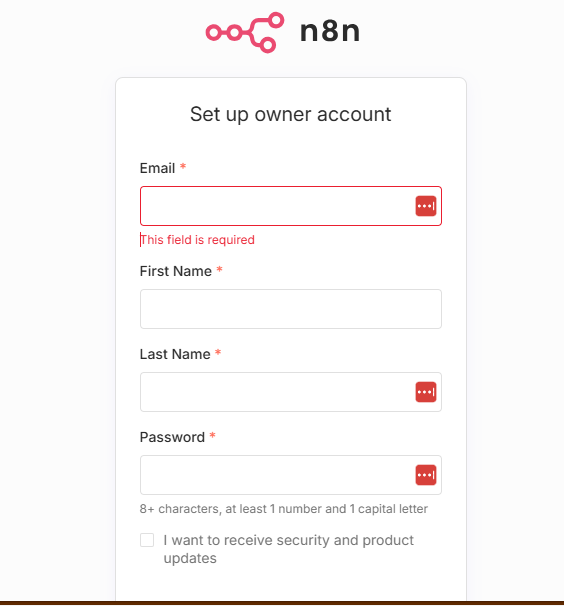
\includegraphics[width=0.55\textwidth]{Figures/n8n-localhost-5678-success-2026-04-25.png}
    \caption{Local n8n runtime verification at localhost port 5678.}
    \label{fig:appendix-n8n-runtime-proof}
\end{figure}

Figure~\ref{fig:appendix-detailed-final-architecture} shows the detailed architecture diagram kept as supporting evidence.

\begin{figure}[H]
    \centering
    \makebox[\textwidth][c]{%
        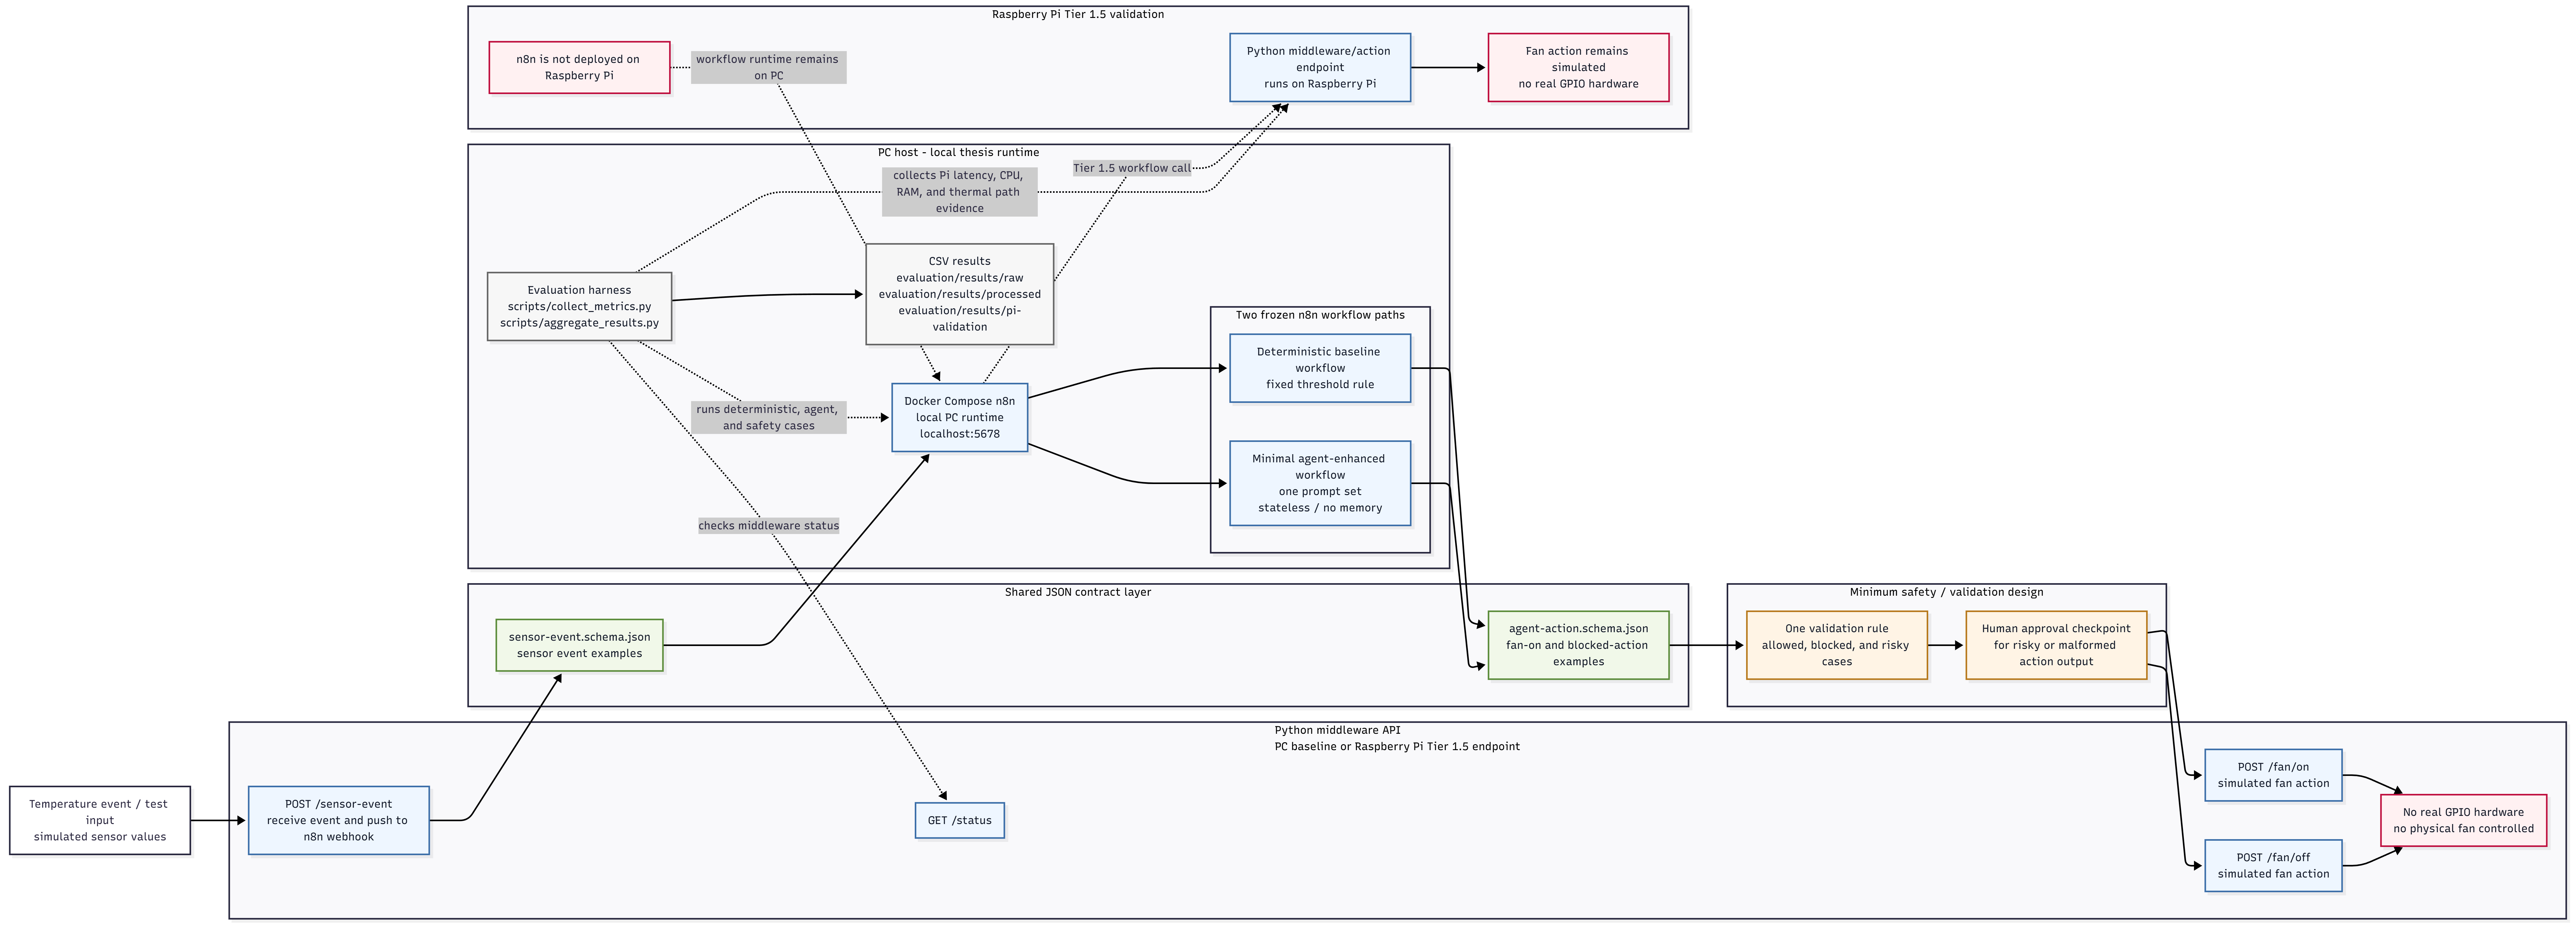
\includegraphics[width=1.08\textwidth]{Figures/appendix-detailed-final-architecture.png}%
    }
    \caption{Detailed architecture diagram preserved as supporting evidence.}
    \label{fig:appendix-detailed-final-architecture}
\end{figure}

Figure~\ref{fig:appendix-pi-middleware-cpu-ram} shows the Raspberry Pi middleware CPU and RAM observation used as supporting resource evidence.

\begin{figure}[H]
    \centering
    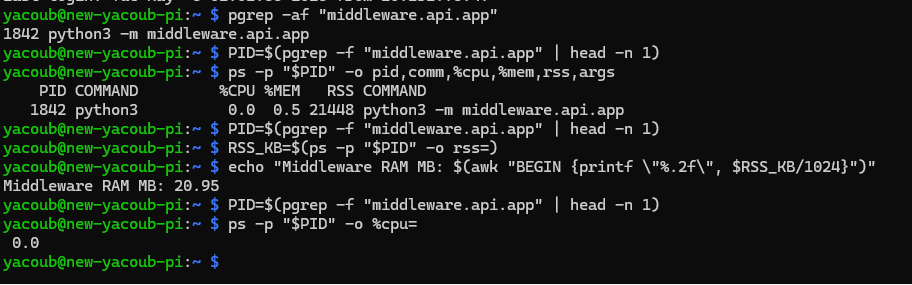
\includegraphics[width=0.95\textwidth]{Figures/appendix-pi-middleware-cpu-ram.png}
    \caption{Raspberry Pi middleware CPU and RAM observation.}
    \label{fig:appendix-pi-middleware-cpu-ram}
\end{figure}

Figures~\ref{fig:appendix-pi-terminal-high-temp-fan-on} and~\ref{fig:appendix-pi-terminal-low-temp-fan-off} show terminal evidence for the Raspberry Pi high- and low-temperature validation cases.

\begin{figure}[H]
    \centering
    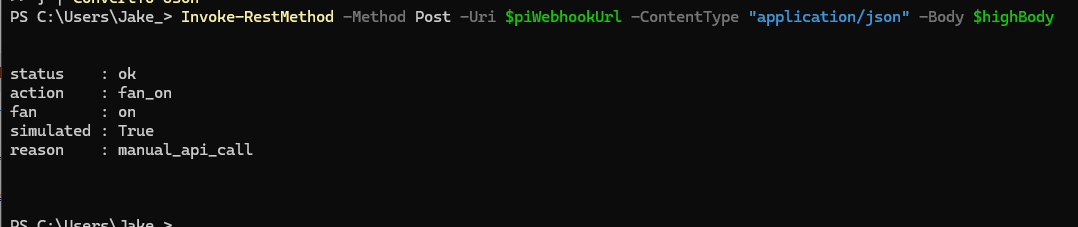
\includegraphics[width=0.95\textwidth]{Figures/appendix-pi-terminal-high-temp-fan-on.png}
    \caption{Raspberry Pi terminal evidence for the high-temperature fan-on case.}
    \label{fig:appendix-pi-terminal-high-temp-fan-on}
\end{figure}

\begin{figure}[H]
    \centering
    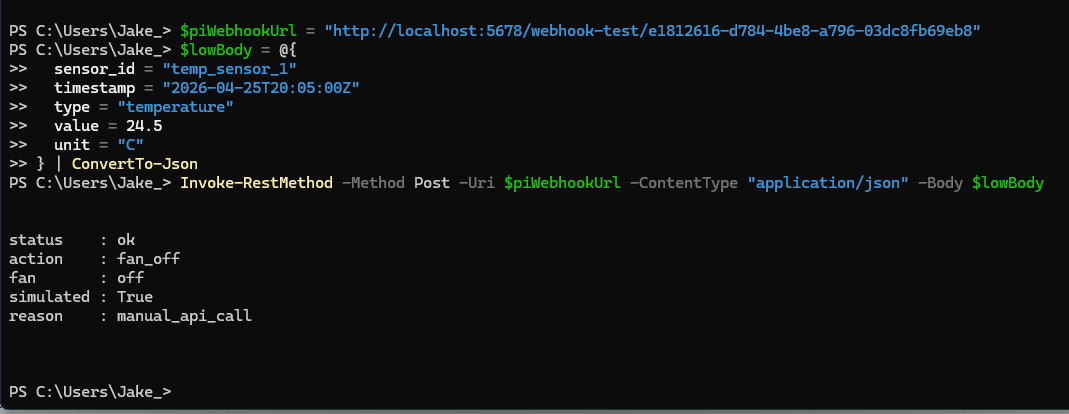
\includegraphics[width=0.95\textwidth]{Figures/appendix-pi-terminal-low-temp-fan-off.png}
    \caption{Raspberry Pi terminal evidence for the low-temperature fan-off case.}
    \label{fig:appendix-pi-terminal-low-temp-fan-off}
\end{figure}

\end{document}
